\documentclass[11pt, a4paper]{article}
\usepackage[nochapters]{classicthesis}
\usepackage[margin=42mm]{geometry}
\usepackage[utf8]{inputenc}
\usepackage[T1]{fontenc}
\usepackage{graphicx}
\usepackage{url}
\usepackage{multirow}
\usepackage{amsfonts}
\usepackage{amsmath}
\usepackage{nicefrac}
\usepackage{microtype}
\usepackage{float}
\usepackage{algorithm}
\usepackage{algpseudocode}

\usepackage{geometry}    % Required to adjust page margins
\usepackage{xltabular}   % Replaces ltablex for robust multi-page tabularx
\usepackage{booktabs}
\usepackage{array}
\usepackage{changepage}

\usepackage{amssymb}
\usepackage{makecell}

%   \usepackage{xltabular}   % Replaces ltablex for robust multi-page tabularx
%   \usepackage{booktabs}
%   \usepackage{array}
% ─────────────────────────────────────

% \usepackage{tabularx}
% \usepackage{xcolor}    % for \rowcolor
% \usepackage{array}     % for >{\centering\arraybackslash}
% \usepackage{longtable}
% \usepackage{calc}      % needed for \dimexpr arithmetic

% \usepackage{ltablex}
% \keepXColumns

\usepackage{amsthm}
\newtheorem{assumption}{Assumption}
\newtheorem{theorem}{Theorem}

% ... in your document ...
% Define theorem-like environments
\newtheorem{lemma}{Lemma}
\newtheorem{proposition}{Proposition}
\newtheorem{corollary}{Corollary}
\newtheorem{definition}{Definition}

\theoremstyle{remark}
\newtheorem*{remark}{Remark}
\newtheorem*{note}{Note}



\definecolor{darkblue}{rgb}{0, 0, 0.5}
\hypersetup{colorlinks=true,citecolor=darkblue,
            linkcolor=darkblue, urlcolor=darkblue}

\def\thesistitle{Gradient Projection Methods for Continual Learning in Hypernetworks}
\def\subtitle{Overcoming Chunk-Induced Gradient Pathologies via Projection Normalization, and the Introduction of iFOPNG}
\def\yourname{Jakub Michałowski}
\def\yourprogramme{Cognitive Science \& Artificial Intelligence}
\def\yourstudentnumber{u253954}
\def\finalmonth{May}
\def\finalyear{2026}
\def\supervisor{dr. Giacomo Spiegler}
\def\committee{dr. The Second Reader}
\def\acknowledgments{The author thanks dr.\ Giacomo Spiegler for supervision and feedback throughout this project.}
\def\wordcount{$\approx$8500}

\hypersetup{pdfauthor   = \yourname,
            pdftitle    = \thesistitle\ \subtitle,
            pdfsubject  = \yourprogramme\ Bachelor Thesis
}


\usepackage[natbibapa]{apacite}
\bibliographystyle{apacite}

\begin{document}
\input{frontmatter.tex}

\begin{abstract}
    This thesis addresses the fundamental incompatibility of applying gradient
    projection-based continual learning (CL) methods to hypernetwork architectures,
    establishing a novel framework for stable subspace optimization.  Traditional 
    projection methods collapse under hypernetwork architectures: the architectural 
    necessity of weight-chunking forces the model to accumulate an exceptionally large 
    gradient volume before a single projection step can execute, blowing up the condition
    number of the projection matrix and causing catastrophic inversion failures that 
    standard regularisation cannot rescue.
    
    The primary research objective is to eliminate these numerical singularities and
    systematically evaluate whether combining hard geometric projections on top of
    task-conditioned hypernetworks and their output-scoped functional regularizers
    yields a constructive synergy.  To achieve this, we introduce
    \emph{projection-scoped normalization}: gradient columns stored in the memory
    matrix $G$ are rescaled to unit $\ell_2$ norm, and the diagonal empirical Fisher
    vector is rescaled by its absolute maximum, together stabilizing the metric tensor
    within the local projection algebra.  We also introduce \texttt{iFOPNG}, an inertial
    variant of Fisher-Orthogonal Projected Natural Gradient Descent \citep{garg_fisher-orthogonal_2026}
    that replaces the current-task Fisher $F_{\text{new}}$ with the combined curvature
    $F_c = F_{\text{new}}+F_{\text{old}}$, inspired by the parameter-inertia concept
    of Elastic Weight Consolidation.  Methods are benchmarked on sequential Split and Permuted MNIST
    , Split-CIFAR10 and Split-CIFAR100. The empirical findings reveal that projection normalization
    resolves matrix inversion collapse in the tested configurations, and that \texttt{iFOPNG} consistently 
    outperforms \texttt{FOPNG} across all benchmarks; in the standard-capacity hypernetwork
    setting only \texttt{iFOPNG} surpasses plain \texttt{SGD}, while most other projection 
    variants fall below it.  A standalone hypernetwork optimized
    with \texttt{Adam} and \citeauthor{oswald_continual_2020}'s functional regularizer
    consistently surpasses all projection variants, indicating that momentum, which
    projection methods forgo by design, is the decisive factor in compressed generative
    weight spaces.
\end{abstract}



\section{Data Source, Ethics, Code, and Technology Statement}
\label{sec:dsect}

\noindent\textbf{Data Source.} The MNIST (owned by LeCun et al.) and CIFAR (CIFAR-10 and CIFAR-100, owned by Krizhevsky et al.) datasets are public, anonymized datasets licensed for research. These datasets form the basis for the Split-MNIST, Permuted MNIST, Split-CIFAR10, and Split-CIFAR100 benchmarks evaluated in this work. No human or animal data was collected. Data was acquired via the \texttt{torchvision.datasets} API.

\paragraph{Figures.} All figures and plots were created entirely by the author using \texttt{matplotlib} and Weights \& Biases.

\paragraph{Code.} The baseline FOPNG framework was adapted from \citet{garg_fisher-orthogonal_2026}; all other execution infrastructure was implemented by the author (\url{https://github.com/kelares/HyperFisher}). Libraries used: Python (v3.10), PyTorch (v2.x), Torchvision, Weights \& Biases, NumPy, Matplotlib, and Tqdm.

\paragraph{Technology.} The manuscript was typeset in \LaTeX{} using BibTeX. During the preparation of this work, the author(s) used Gemini and Claude in order to optimize academic phrasing, outline structure, paraphrase transitions, and check grammar. After using these tools/services, the author(s) reviewed and edited the content as needed and take(s) full responsibility for the content of the thesis. AI Citations: Google. (2026). \textit{Gemini} [Large language model]. https://gemini.google.com; Anthropic. (2026). \textit{Claude} [Large language model]. https://claude.ai.

\section{Introduction}
\label{sec:introduction}

The capacity for continuous, sequential adaptation without the eradication of
historical knowledge remains an architectural cornerstone of biological
intelligence, yet it presents a fundamental barrier for artificial neural
networks. In deep learning paradigms, sequential training across non-stationary
data distributions triggers a systemic pathology known as \emph{catastrophic
forgetting} \citep{mccloskey_catastrophic_1989}. When a network optimizes its
parameters for an incoming task, gradient updates blindly overwrite the weight
configurations essential for retaining prior task spaces, shifting the internal
representation manifolds away from historical objective minima.

Modern continual learning (CL) literature is conventionally structured into
three core algorithmic families: replay-based strategies that leverage episodic
data buffers, regularization-based frameworks that penalize parameter deviations,
and architectural or parameter-isolation methods \citep{de_lange_continual_2022}.
Within the meta-learning domain, hypernetworks \citep{ha_hypernetworks_2016}
have emerged as an elegant paradigm. Hypernetworks circumvent parameter-space
conflicts by utilizing a centralized, lightweight meta-model to generate the
target network's complete parameter weights conditioned on task embeddings, as
formalized by \citet{oswald_continual_2022}. Concurrently, within the field of
geometric optimization, gradient projection methods---exemplified by the
recently proposed Fisher-Orthogonal Projected Natural Gradient Descent (FOPNG)
\citep{garg_fisher-orthogonal_2026}---explicitly constrain subsequent updates to
the null-space of historical parameter spaces.

Despite the mathematical elegance of both hypernetworks and gradient projection
methods, their structural intersection uncovers a critical and previously
unexamined optimization pathology. To prevent a catastrophic parameter explosion
within the meta-model, a hypernetwork must use sequential weight-chunking.
Depending on the dimensional footprint of the target architecture, this
constraint forces the target model to be produced in hundreds or thousands of
individual sub-blocks. Executing this spawning mechanism prior to a single
backward pass accumulates gradients additively, resulting in parameter gradients
of exceptionally high magnitude. This explosion numerically erases the stabilizing
effect of $\lambda$ during matrix inversion, inflating the condition number of
the projection kernel to extreme scales (e.g., exceeding $10^{10}$) and inducing
catastrophic projection failures.

\subsection*{Research Objectives and Algorithmic Framework}

The primary research objective of this thesis is to systematically resolve this
linear-algebraic collapse, map the initialization mechanics of meta-projection
pipelines, and evaluate whether the integration of hard geometric constraints on
top of soft functional regularizers yields an optimized sequential learning system.

To achieve this, we introduce projection-scoped normalization (column-wise
$\ell_2$ orthonormalization of $G$ combined with absolute-maximum scaling of
$\hat{F}$), an \texttt{AdamW} first-task initialization protocol, and
\texttt{iFOPNG}---an inertial FOPNG variant using the combined metric
$F_c = \hat{F}_{\mathrm{new}} + \hat{F}_{\mathrm{old}}$.  These contributions
enable stable gradient projection in chunked hypernetworks, with direct
applicability to on-device sequential learning where retaining adaptive momentum
is critical.

\subsection*{Research Questions}

To systematically navigate these boundaries, this thesis addresses the following
primary research question:
\begin{quote}
\emph{To what extent can gradient projection methods be successfully integrated
into chunked hypernetwork architectures for continual learning, and how do their
structural pathologies, initialization protocols, and inertial variants impact
optimization efficiency?}
\end{quote}
This is decomposed into four sub-research questions (Sub-RQs):
\begin{itemize}
    \item[\textbf{Sub-RQ1}] \textbf{(Synergy vs.\ Conflict):} Does the joint integration
    of gradient projection frameworks and soft output-scoped functional
    regularization yield a constructive synergy, or does a standalone regularized
    hypernetwork offer a more efficient optimization frontier?
    \item[\textbf{Sub-RQ2}] \textbf{(Gradient Pathology):} How does the architectural
    necessity of spawning thousands of sequential weight-chunks impact gradient
    magnitudes, and to what extent can local projection-scoped normalization
    prevent the resulting explosion from collapsing the matrix inversion?
    \item[\textbf{Sub-RQ3}] \textbf{(Parameter Inertia):} To what degree does
    evaluating the natural gradient projection under a joint Riemannian metric
    ($F_c = \hat{F}_{\mathrm{new}} + \hat{F}_{\mathrm{old}}$), rather than the task-specific
    metric ($\hat{F}_{\mathrm{new}}$) used in standard FOPNG, influence task retention?
    \item[\textbf{Sub-RQ4}] \textbf{(Fisher Accumulation):} How should the historical
    component $\hat{F}_{\mathrm{old}}$ be accumulated across tasks? Specifically, does
    a non-decaying maximum operator preserve early-task knowledge more
    effectively than an exponential moving average (EMA)?
\end{itemize}

\subsection*{Summary of Empirical Findings}

Projection-scoped normalization completely resolves the matrix inversion
collapse; \texttt{iFOPNG} consistently outperforms \texttt{FOPNG} wherever
inter-task Fisher overlap is substantial; and the MAX accumulation operator is
the preferred hyperparameter-free default.  Critically, normalized projection
methods nonetheless fail to match a hypernetwork optimized via \texttt{Adam}:
the loss of adaptive momentum proves to be the binding constraint in compressed
generative weight spaces.

\section{Related Work}
\label{sec:related_work}

% ─────────────────────────────────────────────────────────────────────────────
\subsection{Continual Learning and the Stability-Plasticity Dilemma}

Modern machine learning systems are predominantly trained on fixed datasets
drawn from a single stationary distribution --- a condition that rarely holds
in deployment, where agents must adapt to non-stationary data streams while
retaining prior knowledge.
The fundamental tension between these two objectives is formalized as the
\emph{stability-plasticity dilemma} \citep{grossberg_how_1980}: an agent must
remain plastic enough to absorb novel distributions yet stable enough to resist
the erasure of established representations.


The continual learning literature addresses this across three canonical
scenarios \citep{de_lange_continual_2022}:
\emph{task-incremental learning}, where the task identity is available at
both training and test time; \emph{class-incremental learning}, where task
identity is withheld at inference; and \emph{domain-incremental learning},
where the output space is shared but the input distribution shifts
continuously.
This thesis focuses on the task-incremental setting, the scenario in which
projection-based methods and hypernetwork architectures have been most
thoroughly evaluated and in which structural comparisons between them are
most tractable.

% % ─────────────────────────────────────────────────────────────────────────────
\subsection{Evaluation Protocols: Multi-Head and Single-Head Designs}
\label{sec:eval_protocols}

Task-incremental benchmarks are evaluated under one of two output-layer
protocols. The \emph{multi-head} protocol gives each task a dedicated output
head, selected by task identity at test time, which removes output-level
interference between tasks; the \emph{single-head} protocol shares one output
layer, forcing the backbone alone to resolve that interference.
\citet{farquhar_towards_2018} showed that multi-head evaluation systematically
inflates apparent method performance by eliminating a major source of
forgetting, and argued that the single-head protocol is the more rigorous
test. Split-MNIST is therefore evaluated under both: the multi-head variant
reproduces the conditions of \citet{garg_fisher-orthogonal_2026} for direct
numerical comparison, and the single-head variant follows
\citet{farquhar_towards_2018} as the harder, more discriminating evaluation.
The exact head configuration and the protocol assigned to each benchmark are
given in Section~\ref{sec:benchmarks}.
% ─────────────────────────────────────────────────────────────────────────────
\subsection{Fisher Information Matrix}
\label{sec:fisher_rw}

Several methods surveyed in this thesis quantify parameter importance through
the \emph{Fisher Information Matrix} (FIM).
For a parametric model $p_\theta(y \mid x)$ with parameters
$\theta \in \mathbb{R}^P$, the FIM is the $P \times P$ matrix
\begin{equation}
    F(\theta)
    = \mathbb{E}_{x \sim q(x)}\,
      \mathbb{E}_{y \sim p_\theta(\cdot \mid x)}
      \Bigl[
        \nabla_\theta \log p_\theta(y \mid x)\,
        \nabla_\theta \log p_\theta(y \mid x)^\top
      \Bigr],
    \label{eq:fim}
\end{equation}
where $q(x)$ is the data-generating distribution \citep{amari_natural_1998}.
$F(\theta)$ defines a Riemannian metric on the parameter manifold: the
Fisher inner product $\langle u, v\rangle_F = u^\top F(\theta)\,v$ measures
distances in terms of the change in model predictions, not in terms of raw
Euclidean parameter displacement.

The full FIM is intractable at the scale of neural networks.
All methods evaluated in this thesis use the \emph{diagonal empirical
approximation}, which replaces the outer-product expectation with an
empirical average over $N$ observed data points:
\begin{equation}
    \hat{F}_i
    \;\approx\;
    \frac{1}{N}\sum_{n=1}^{N}
    \left(\frac{\partial \mathcal{L}^{(n)}}{\partial \theta_i}\right)^{\!2},
    \label{eq:empirical_fisher}
\end{equation}
yielding a non-negative scalar $\hat{F}_i$ for each parameter $\theta_i$.
The resulting vector $\hat{F} \in \mathbb{R}^P_{\geq 0}$ is treated as a
diagonal matrix in all subsequent quadratic forms.
This approximation reduces storage from $\mathcal{O}(P^2)$ to
$\mathcal{O}(P)$ and is the variant used by EWC
\citep{kirkpatrick_overcoming_2017} and all Fisher-based projection methods
evaluated in \citep{garg_fisher-orthogonal_2026}.

% ─────────────────────────────────────────────────────────────────────────────
\subsection{Regularization-Based Approaches}
\label{sec:rw_regularization}

The dominant paradigm for addressing catastrophic forgetting is
\emph{parameter regularization}, of which Elastic Weight Consolidation (EWC)
\citep{kirkpatrick_overcoming_2017} is the canonical representative.
EWC uses $F_i$ (Equation~\ref{eq:empirical_fisher}) as an importance
weight for each parameter, and applies a soft quadratic penalty that resists
changes to parameters deemed important to prior tasks:
\begin{equation}
\label{eq:ewc}
    \mathcal{L}_{\mathrm{EWC}}(\theta)
    = \mathcal{L}_t(\theta)
    + \frac{\lambda}{2}\sum_i F_i
      \bigl(\theta_i - \theta_{t-1,i}^*\bigr)^2,
\end{equation}
where $\theta \in \mathbb{R}^p$ are the model parameters,
$\theta^*_{t-1}$ is their snapshot saved after task $t{-}1$,
and $\lambda > 0$ governs overall regularization strength.
EWC is computationally efficient and broadly applicable, and serves as the
standard reference point against which new continual learning methods are
measured.
Its principal limitation is that soft penalties permit bounded parameter
drift: cumulative updates across a long task sequence gradually erode the
protection of earlier task spaces, a failure mode that becomes increasingly
pronounced as $T$ grows \citep{de_lange_continual_2022}.

% ─────────────────────────────────────────────────────────────────────────────
\subsection{Gradient Projection Methods}
\label{sec:rw_projection}

To enforce strict, non-negotiable protection for prior knowledge rather than
relying on penalties that can be overcome by sufficiently large gradients,
a second paradigm uses explicit \emph{gradient projection}.
Orthogonal Gradient Descent (OGD) \citep{farajtabar_orthogonal_2019} maintains
a memory matrix $G = [g_1 \mid \cdots \mid g_K] \in \mathbb{R}^{p \times K}$
of historical task gradient directions and projects incoming gradients onto the
orthogonal complement of $\operatorname{Col}(G)$ before each parameter update:
\begin{equation}
    \tilde{g} = g - G(G^\top G)^{-1}G^\top g.
\end{equation}
This provides a hard guarantee: the projected update cannot increase the loss
on any previously seen task.
Generalization bounds established within the Neural Tangent Kernel regime
confirm that OGD provides exact protection in linear and mildly nonlinear
settings \citep{bennani_generalisation_2020}.

However, standard Euclidean projection treats the parameter space as flat,
assigning equal importance to all directions regardless of the curvature of
the loss surface.

Fisher-Orthogonal Projected Natural Gradient Descent (FOPNG)
\citep{garg_fisher-orthogonal_2026} addresses this by performing the
projection in the Riemannian geometry defined by $\hat{F}$, the diagonal
empirical Fisher of the current task, so that the orthogonality constraint
respects the local curvature of the loss surface.
The related Fisher Natural Gradient (FNG) \citep{garg_fisher-orthogonal_2026}
applies the natural gradient without any projection, and Orthogonal Natural
Gradient (ONG) \citep{yadav_ong_2025} combines Fisher preconditioning with
Euclidean projection, sitting structurally between OGD and FOPNG.
Exact algorithmic instantiations are given in Section~\ref{sec:projection_methods}.

% ─────────────────────────────────────────────────────────────────────────────
\subsection{Hypernetworks for Continual Learning}
An orthogonal architectural response to catastrophic forgetting replaces the
multi-head output design entirely with a \emph{hypernetwork}
\citep{ha_hypernetworks_2017}: a meta-model
$\mathcal{H}(\cdot;\phi)$ trained to synthesize the complete weight
vector $\theta_t = \mathcal{H}(e_t;\phi)$ of a target network,
conditioned on a task embedding $e_t$.
Each task receives a unique weight configuration generated on demand, rather
than a dedicated output head, achieving implicit task separation through the
generative bottleneck.

Generating the full $\theta_t$ in a single forward pass is computationally
intractable for large target networks, so \citet{oswald_continual_2020}
introduced \emph{weight chunking}: the generator iterates over $C$ chunk
embeddings $c_1,\dots,c_C$, producing a fixed-size block of target parameters
per pass and concatenating them into the full weight vector $\theta_t$.
To prevent the hypernetwork from forgetting how to generate the weights of
earlier tasks, a soft \emph{functional regularizer} anchors the generator in
its own output space.
Let $\theta_s = \mathcal{H}(e_s;\phi)$ be the target-network weight vector the
generator currently produces for task $s$ under the single, evolving parameter
set $\phi$.
On completion of task $s$, the generated vector is cached as a fixed reference
$\theta^{\mathrm{ref}}_s$, detached from the computation graph.
While task $t$ is trained, only $\phi$ is updated, and every reference
$\{\theta^{\mathrm{ref}}_s\}_{s<t}$ stays fixed at the value it held when its
task finished, under the penalty
\begin{equation}
    \mathcal{L}_{\mathrm{reg}}
    = \frac{\beta}{t-1} \sum_{s=1}^{t-1}
      \bigl\| \mathcal{H}(e_s;\phi) - \theta^{\mathrm{ref}}_s \bigr\|_2^2,
\end{equation}
with regularization strength $\beta > 0$.
The penalty therefore measures, in the space of generated weights, how far the
current generator has drifted from the exact target parameters it once produced
for each past task.
This can be interpreted as EWC applied at the meta level: rather than anchoring individual target
parameters, it anchors the generated weight configurations for each previously
seen task, penalising drift in the function space where task-relevant
quantities actually live.
% ──────────────────
\subsection{Identified Gaps and Motivating Pathologies}

Whether hard geometric projection constraints are compatible with the
soft functional regularization already employed by hypernetworks, or
whether layering both simultaneously over-constrains the generator's
plasticity, has not been investigated (Sub-RQ1).

The architectural necessity of weight-chunking introduces a
gradient accumulation pathology --- inflated condition numbers in
the projection kernel --- that is unique to the hypernetwork and projection methods combination
and has no prior treatment in the literature (Sub-RQ2).

Existing Fisher-based projection methods define the projection geometry from a
single-task Fisher metric, which does not weight parameters by their importance
to past tasks; whether replacing it with a combined metric
$F_c = F_{\mathrm{new}} + F_{\mathrm{old}}$ that anchors historically important
coordinates, giving them inertia, yields consistent retention improvements
across benchmarks has not been examined (Sub-RQ3).

The historical Fisher estimate underlying Fisher-based projection
depends on a choice of accumulation operator; whether a monotonic
maximum or a decaying exponential moving average better preserves
long-horizon retention has not been directly compared (Sub-RQ4).

% ─────────────────────────────────────────────────────────────────────────────
% METHODOLOGY SECTION --- clean rewrite
% Principles:
%   - Operational focus: equations + implementation choices, not re-introduction
%   - Related Work already introduced EWC, OGD, FOPNG, HN conceptually
%   - Novel contributions (iFOPNG, normalization, dropout decision) get full
%     treatment; baselines get equations + key parameters only
%   - ONG and FNG filled in from Garg et al. (2026) formulations
%   - Dropout paragraph cleaned of HTML rendering artifacts
% ─────────────────────────────────────────────────────────────────────────────

\section{Methods}
\label{sec:methods}
% ─────────────────────────────────────────────────────────────────────────────
\subsection{Continual Learning Protocol}
\label{sec:cl_protocol}

\subsubsection{Task Setup and Evaluation Metrics}
A continual learning agent receives a sequence of $T$ tasks
$\mathcal{T}_1, \mathcal{T}_2, \ldots, \mathcal{T}_T$ presented in order.
At task $t$, only the data from $\mathcal{T}_t$ is available; prior task
data is not retained.
After each task is trained, the model is evaluated on all tasks seen so far.
We report two aggregate metrics: \emph{average accuracy}
\begin{equation}
    A_t = \frac{1}{t}\sum_{i=1}^{t} a_{t,i},
\end{equation}
and \emph{backward transfer}
\begin{equation}
    \mathrm{BWT} = \frac{1}{T-1}\sum_{t=2}^{T}(a_{T,t}-a_{t,t}),
\end{equation}
where $a_{i,j}$ denotes accuracy on task $j$ immediately after training
task $i$.
Negative BWT quantifies catastrophic forgetting; a value of zero indicates
perfect retention.

Reporting both metrics jointly is necessary because each can mask
failure modes invisible to the other: a method that forecloses new
learning to preserve old tasks achieves near-zero BWT alongside collapsed
accuracy, while a method that overfits each new task sustains competitive
accuracy at the cost of large negative BWT on earlier ones.

% ─────────────────────────────────────────────────────────────────────────────
\subsection{Fisher Information Matrix and Regularization-Based Continual Learning}
\label{sec:fisher_ewc}

All Fisher-based methods evaluated in this thesis use the diagonal empirical
approximation $F$ defined in Equation~\eqref{eq:empirical_fisher}.
The $F_{\mathrm{new}}$ and $F_{\mathrm{old}}$ used in
projection methods denote the FIMs computed from the current task's data and
accumulated from all prior tasks, respectively; both are instances of Equation~\eqref{eq:empirical_fisher}.

\subsubsection{Elastic Weight Consolidation}
\label{sec:ewc}
EWC (Section~\ref{sec:rw_regularization}, Equation~\ref{eq:ewc}) is included as
a regularization baseline that operates purely through parameter-space
penalties and maintains no gradient subspace.
We use $\lambda = 10^{-3}$ for all hypernetwork configurations and
reproduce the per-benchmark values from \citet{garg_fisher-orthogonal_2026}
Table~1 for standalone evaluations.
Fisher estimates are computed over the full training set for MNIST-based
benchmarks and over $N{=}1024$ samples for CIFAR benchmarks.

% ─────────────────────────────────────────────────────────────────────────────
\subsection{Gradient Projection Methods}
\label{sec:projection_methods}

This subsection presents the full suite of gradient-based methods evaluated
in this thesis.
\texttt{SGD} and \texttt{FNG} establish unconstrained lower bounds with no
forgetting-protection mechanism; \texttt{OGD} through \texttt{iFOPNG} form
the projection family that is the primary focus of this work.
% Basic learning algorithm
\subsubsection{Stochastic Gradient Descent}
\texttt{SGD} applies vanilla gradient descent with no forgetting protection:
\begin{equation}
    \Delta\theta_{\mathrm{SGD}} = -\eta\,\nabla_\theta\mathcal{L}_t.
\end{equation}
\texttt{Adam} \citep{kingma_adam_2015} is included as an adaptive-rate
variant that maintains per-parameter momentum; both serve as unconstrained
baselines.

% Basic projection, Euclidean space
\subsubsection{Orthogonal Gradient Descent}
\label{sec:ogd}
OGD \citep{farajtabar_orthogonal_2019} maintains a memory matrix
$G = [g_1 \mid \cdots \mid g_K] \in \mathbb{R}^{p \times K}$ of past task
gradient directions and updates parameters via the current gradient
projected onto the orthogonal complement of $\operatorname{Col}(G)$:
\begin{equation}
    \tilde{g} = g - G(G^\top G)^{-1}G^\top g,
    \qquad
    \Delta\theta_{\mathrm{OGD}} = -\eta\,\tilde{g}.
\end{equation}

\paragraph{Gradient memory management.}
In all projection methods, $G$ is maintained as a fixed-budget basis of at most $M$ columns; 
insertion, orthonormalisation, and overflow recompression are detailed in Section~\ref{sec:normalization}.

% Riemannian step without projection
\subsubsection{Natural Gradient and Fisher Natural Gradient}
Natural gradient descent \citep{amari_natural_1998} replaces the Euclidean
gradient step with one measured in the Riemannian geometry of the Fisher
metric, so that equal step sizes correspond to equal changes in model
predictions rather than equal changes in parameter values:
\begin{equation}
    \Delta\theta_{\mathrm{nat}} = -\eta\,F^{-1}_{\mathrm{new}}\nabla_\theta\mathcal{L}.
\end{equation}
\texttt{FNG} \citep{garg_fisher-orthogonal_2026} applies a trust-region
constraint to this step, normalising by the Fisher norm of the gradient:
\begin{equation}
    v^*_{\mathrm{FNG}}
    = -\eta\,\frac{F^{-1}_{\mathrm{new}} g}
                  {\sqrt{g^\top F^{-1}_{\mathrm{new}} g}}.
\end{equation}
FNG maintains no gradient subspace and provides no forgetting protection;
it is included to isolate the contribution of Fisher preconditioning
independently of projection.

% OGD projection applied to the natural gradient step
\subsubsection{Orthogonal Natural Gradient}
ONG \citep{yadav_ong_2025} extends OGD by replacing the raw gradient with
the natural gradient before projection.
The natural gradient $F^{-1}_{\mathrm{new}}g$ is first computed, then
projected onto the Euclidean orthogonal complement of $\operatorname{Col}(G)$:
\begin{equation}
    \Delta\theta_{\mathrm{ONG}}
    = -\eta\!\left(
        F_{\mathrm{new}}^{-1}g
        - G(G^\top G)^{-1}G^\top F_{\mathrm{new}}^{-1}g
    \right).
\end{equation}
The step direction is Fisher-preconditioned, but the orthogonality
constraint is still measured in Euclidean space: the kernel being
inverted is $A = G^\top G + \lambda I$, identical to OGD.
Following the diagonal Fisher approximation used throughout this thesis,
we substitute the EKFAC inverse of \citet{yadav_ong_2025} with the
diagonal empirical Fisher; results are not directly comparable to the % ITS ALREADY STATED SOMEWHERE
original implementation.

% Both step and projection in Riemannian space
\subsubsection{Fisher-Orthogonal Projected Natural Gradient Descent}
\texttt{FOPNG} \citep{garg_fisher-orthogonal_2026} moves both the step
and the projection into the Riemannian geometry of the Fisher metric.
Where ONG projects the natural gradient in Euclidean space, FOPNG measures
orthogonality in Fisher space: a direction is orthogonal to the stored
basis if it produces no change in model predictions along those directions,
not merely no change in parameter values.
The constrained trust-region update is:
\begin{equation}
    v^*_{\mathrm{FOPNG}} = -\eta\,
    \frac{F^{-1}_{\mathrm{new}} Pg}{\sqrt{(Pg)^\top F^{-1}_{\mathrm{new}} Pg}},
    \qquad
    P = I - F_{\mathrm{old}}\, G\!\left(G^\top F_{\mathrm{old}}\,
        F^{-1}_{\mathrm{new}} F_{\mathrm{old}}\, G
        + \lambda I\right)^{\!-1}\! G^\top F_{\mathrm{old}},
    \label{eq:fopng}
\end{equation}
where $F_{\mathrm{new}}$ is the current-task empirical Fisher,
$F_{\mathrm{old}}$ is the accumulated historical Fisher under which the
stored directions were collected, and $\lambda I$ is a damping term for
numerical stability.
This is the pre-Fisher form of \citet{garg_fisher-orthogonal_2026}, in
which the stored basis carries its collection-time Fisher weighting.

% Single substitution: F_new -> F_c
\subsubsection{Inertial FOPNG}
\label{sec:ifopng}

In FOPNG the Riemannian metric governing both the trust-region constraint
and the projection objective is $F_{\mathrm{new}}$ alone.
This is natural on the first task but creates an asymmetry as history
accumulates: the subspace $\operatorname{Col}(G)$ encodes directions
important to prior tasks, yet the metric assigns zero curvature to
parameters that were important previously but are uninformative on the
current task, allowing the update to move freely through historically
sensitive directions.

\texttt{iFOPNG} resolves this asymmetry by replacing $F_{\mathrm{new}}$
with the \emph{combined metric}
\begin{equation}
    F_c \;\coloneqq\; F_{\mathrm{new}} + F_{\mathrm{old}},
    \label{eq:combined_fisher}
\end{equation}
where $F_{\mathrm{old}}$ is maintained as the element-wise maximum of all
per-task Fisher diagonals accumulated so far.
Substituting $F_c$ for $F_{\mathrm{new}}$ throughout
Equation~\eqref{eq:fopng} yields:
\begin{equation}
    v^* = -\eta\,
    \frac{F_c^{-1}Pg}{\sqrt{(Pg)^\top F_c^{-1}Pg}},
    \qquad
    P = I - F_{\mathrm{old}}\,G\,A^{-1}\,G^\top F_{\mathrm{old}},
    \label{eq:ifopng}
\end{equation}
where $A = G^\top F_{\mathrm{old}}\,F_c^{-1}\,F_{\mathrm{old}}\,G
+ \lambda I$.
This update is derived as the closed-form solution of the trust-region
projection problem in Theorem~\ref{thm:ifopng}
(Appendix~\ref{app:a}).

The combined metric assigns each coordinate $i$ an effective curvature
$(F_{\mathrm{new}})_i + (F_{\mathrm{old}})_i$, suppressing the step size
in directions important to any task in the sequence.
We call this \emph{parameter inertia}: a coordinate that accumulated high
Fisher importance is not pulled back toward a stored reference point ---
it is made harder to displace.
This contrasts with EWC \citep{kirkpatrick_overcoming_2017}, which achieves
retention through an explicit quadratic penalty anchored at $\theta^*$;
\texttt{iFOPNG} achieves it geometrically, through the ambient metric alone.

% ─────────────────────────────────────────────────────────────────────────────
\subsection{Hypernetwork Architecture}
\label{sec:hn_arch}

\subsubsection{Chunked Hypernetworks}
Generating $\theta_t$ in a single forward pass would require an output
layer of dimension $|\theta_t|$, which is computationally prohibitive for
any non-trivial target architecture.
\emph{Weight chunking} \citep{oswald_continual_2020} resolves this by
iterating over a secondary chunk embedding $c_k$, $k=1,\ldots,K$,
and producing a block of $C_s$ target parameters per pass; the full weight
vector is assembled by concatenation.
Chunking makes the hypernetwork parameter-efficient but introduces the
chunk-induced gradient accumulation pathology addressed in
Section~\ref{sec:normalization}.

\subsubsection{Functional Regularizer}
The functional regularizer of \citet{oswald_continual_2020} is active for
all hypernetwork configurations, with regularization strength $\beta$ treated
as a tunable hyperparameter (see Appendix~\ref{app:hyperparameters}).

\subsubsection{Target Network and Dropout}
\label{sec:dropout}
Standalone configurations reproduce the target network architecture of
\citet{garg_fisher-orthogonal_2026} without modification, including two
\texttt{Dropout}$(p{=}0.5)$ layers in the \texttt{SimpleCIFARCNN} classifier
head.
Dropout is removed from the target network in all hypernetwork configurations.
In chunked generation, the hypernetwork executes $K$ sequential forward
passes through the same target architecture before any gradient update;
because all passes share the parent module's training state, stochastic
dropout masks are resampled independently on every chunk pass, injecting
uncontrolled noise into the gradient signal accumulated across chunks.
Removing dropout eliminates this source of variance without modifying
any other aspect of the target architecture
% ─────────────────────────────────────────────────────────────────────────────
\subsection{Novel Algorithmic Contributions}
\label{sec:novel}

\subsubsection{Projection-Scoped Normalization}
\label{sec:normalization}

When a hypernetwork spawns $K$ sequential weight-chunks before a single
projection step executes, the accumulated gradient vector and the diagonal
Fisher entries grow in magnitude proportionally to $K$, inflating the
condition number of the projection kernel $A$ and causing the
matrix inversion in Equation~\eqref{eq:fopng} to fail catastrophically for
any practically sized target network.

We resolve this with two independent rescaling operations that address
distinct sources of ill-conditioning:

\begin{enumerate}
    \item \textbf{Gradient basis orthonormalization.}
        Each batch of $K$ gradient vectors collected after task $t$ is
        replaced by the orthonormal factor $Q$ from its thin QR
        decomposition before insertion into $G$:
        \begin{equation}
            [g_{t,1} \mid \cdots \mid g_{t,K}]
            \;\xrightarrow{\;\mathrm{QR}\;}\; Q,
            \qquad Q^\top Q = I.
        \end{equation}
        QR is chosen over SVD at insertion time because the operation
        requires only orthonormalization of the incoming batch --- the
        number of columns is preserved, not reduced, so the ordered
        factorization that SVD provides is unnecessary overhead.
        SVD is reserved for the overflow handler: when the column count
        of $G$ exceeds the budget $M$, the full basis is recompressed as
        $G \leftarrow U_{:,\,1:M}$, retaining the $M$ left singular
        vectors of greatest variance and discarding the rest.
        This operation applies \emph{at storage time} and affects only
        the basis $G$; the gradient $g$ entering the projection update
        itself is the unmodified parameter gradient from the model.

    \item \textbf{Metric-tensor scaling.}
        Within each projection computation, all Fisher quantities are
        jointly divided by a single scale factor derived from the
        maximum entry of the method's ambient metric $F^*$:
        \begin{equation}
            s = \max\bigl(F^*,\; 1\bigr),
            \qquad
            \tilde{F} = F \,/\, s
            \;\;\text{for } F \in \bigl\{F_{\mathrm{old}},\,
            F_{\mathrm{new}},\, F_c\bigr\},
            \qquad \tilde{\lambda} = \lambda \,/\, s,
            \label{eq:scaling}
        \end{equation}
        where $F^* = F_{\mathrm{new}}$ for \texttt{FNG}, \texttt{ONG},
        and \texttt{FOPNG}, and $F^* = F_c$ for \texttt{iFOPNG}.
        The clamp to 1 prevents division below unity when the Fisher is
        near-zero.
        The damping coefficient $\lambda$ is rescaled by the same factor,
        so its ratio to the Fisher magnitude is held fixed as the absolute
        Fisher scale drifts across tasks. This is necessary because a
        single additive $\lambda$ cannot regularise the kernel by itself
        once chunk accumulation has inflated its spectrum: with the
        smallest and largest eigenvalues of $A$ separated by as much as ten
        orders of magnitude (Section~\ref{sec:results_rq2}), any $\lambda$
        large enough to lift the smallest eigenvalues away from zero
        simultaneously swamps the informative mid-spectrum directions,
        while any $\lambda$ small enough to leave those directions intact
        is negligible against the largest eigenvalues and does nothing for
        the conditioning. Because the condition number is invariant to a
        positive scalar multiple of $A$, the rescaling does not reduce
        $\kappa(A)$ directly; its purpose is to return the absolute
        magnitudes of $A$, its damped inverse, and the trust-region
        denominator to a range in which finite-precision arithmetic
        retains its significant digits and the fixed $\lambda$ acts as a
        meaningful regulariser rather than as numerical noise. 
        % The normalisation is heuristic: it stabilises the inversion of $A$
        % without providing algebraic guarantees on the resulting update % Hmm, maybe thats not needed.
        direction.
\end{enumerate}

Together, these operations ensure that the method-specific projection
kernel $A$ remains well-conditioned regardless of the number of chunks
spawned per task.
The kernel differs structurally across methods:
\begin{equation}
    A =
    \begin{cases}
        G^\top G + \lambda I
            & \text{\texttt{OGD}, \texttt{ONG}} \\[4pt]
        G^\top F_{\mathrm{old}}\,
            F_{\mathrm{new}}^{-1}\,
            F_{\mathrm{old}}\, G + \lambda I
            & \text{\texttt{FOPNG}} \\[4pt]
        G^\top F_{\mathrm{old}}\,
            F_c^{-1}\,
            F_{\mathrm{old}}\, G + \lambda I
            & \text{\texttt{iFOPNG}}
    \end{cases}
    \label{eq:projection_kernel}
\end{equation}
Gradient orthonormalization eliminates column-scale inflation in $G$,
which directly reduces the spectral range of $A$ for all three variants.
Metric-tensor normalization bounds $\tilde{F}$ to $[0,\,1]$, preventing
the Fisher-weighted variants from producing numerically singular $A$.
The \texttt{OGD}/\texttt{ONG} kernel is unaffected by metric-tensor
scaling by construction.
Subspace membership is invariant to positive scalar rescaling of basis
vectors, so neither operation alters the geometry of the projection.

% \paragraph{Principled rescaling and open problem.}
% \label{sec:ng_limitation}
% The proposed normalization --- QR orthonormalization of the gradient basis
% combined with max-entry scaling of $F_c$ --- is heuristic in nature: it
% discards the eigenvalue structure of the pullback metric and applies
% isotropic rather than curvature-aware rescaling to the chunk embedding
% directions.
% The principled alternative is the natural gradient under the Riemannian
% metric induced by the chunk-generating map:
% \begin{equation}
%     \Delta c_i = -\eta\,(J_i^\top J_i + \lambda I)^{-1}\,
%                   \nabla_{c_i}\mathcal{L},
%     \qquad
%     J_i = \frac{\partial W_i}{\partial c_i} \in \mathbb{R}^{C_s \times d_c},
% \end{equation}
% which rescales each chunk embedding direction in proportion to how
% strongly it moves the generated weights, and is tractable because
% $d_c \ll C_s$.
% This preconditioner was implemented and evaluated experimentally.
% Applied to the raw gradient \emph{prior} to the projection step, it
% consistently degraded continual learning performance --- BWT worsened by
% approximately $0.33$ on Split-MNIST SH relative to the heuristic baseline.
% We attribute this to a metric mismatch: the FOPNG projection operator is
% calibrated for gradients in Euclidean parameter space, and preconditioning
% only the chunk embedding component before projection produces a
% geometrically inconsistent input to the kernel $G^\topFG$.
% The principled resolution --- applying $(J_i^\top J_i + \lambda I)^{-1}$
% to the projected update $v^*$ rather than to the raw gradient, so that the
% projection sees Euclidean gradients and the Riemannian step follows --- is
% left to future work.

% ─────────────────────────────────────────────────────────────────────────────
% Experimental Design
% Now a \subsection of the Methods section (fits the fixed thesis structure).
%
% Hyperparameter provenance: benchmark-specific values deferred to the
% appendix table.
% ─────────────────────────────────────────────────────────────────────────────

\subsection{Experimental Design}
\label{sec:experimental_design}

The four sub-research questions demand qualitatively different experimental
designs. Sub-RQ1 and Sub-RQ3 require head-to-head benchmark comparisons ---
projection methods against an unconstrained baseline, and \texttt{iFOPNG}
against \texttt{FOPNG} respectively. Sub-RQ2 requires a controlled ablation
over normalization conditions. Sub-RQ4 requires a long-horizon comparison of
two Fisher accumulation operators on the same inertial combined-metric preconditioner.

% ─────────────────────────────────────────────────────────────────────────────
\subsubsection{Hyperparameter Provenance}
\label{sec:hparam_provenance}

\paragraph{Standalone target-network experiments.}
All hyperparameter values for experiments without a hypernetwork ---
learning rates, regularization coefficients, gradient budgets, Fisher
sample counts, batch sizes, and epoch counts --- are taken without
modification from \citet{garg_fisher-orthogonal_2026} Table~1.
\texttt{iFOPNG} uses the same values as \texttt{FOPNG}, since the inertial
combined Fisher introduces no hyperparameters beyond those FOPNG already
defines.
\texttt{ONG} \citep{yadav_ong_2025} is treated as a composite
method: it applies \texttt{OGD}'s Euclidean projection operator to the
natural gradient direction and introduces no hyperparameters beyond those
already specified for \texttt{OGD} and \texttt{FNG}; its values therefore
follow \texttt{OGD}'s Table~1 entries.

\paragraph{Deviation for first-task initialization.}
We deviated from the original protocol in one specific instance: first-task 
initialization for MNIST-based benchmarks. While \citet{garg_fisher-orthogonal_2026} 
state they used the method's own learning rate for first-task SGD training 
(e.g., $\eta = 10^{-5}$ for FOPNG), our empirical replication of this protocol 
yielded an initial accuracy of only $\approx 21\%$. As demonstrated by the 
learning rate convergence sweep detailed in Appendix~D (Figure~\ref{fig:sgd_threshold}), 
this published rate falls well below the empirical convergence threshold, 
effectively failing to establish a functional baseline. To ensure a clean initial 
projection subspace, we standardized the first-task SGD learning rate to $10^{-3}$ 
for MNIST-based benchmarks and $10^{-2}$ for CIFAR-based benchmarks. 
Beyond this necessary empirical correction, no tuning was performed on the published values.

\paragraph{Hypernetwork experiments.}
Settings not covered by \citet{garg_fisher-orthogonal_2026} follow the canonical 
hypernetwork framework of \citet{oswald_continual_2020}; exact values are detailed 
in Appendix~\ref{app:hyperparameters}. Because computing a full Fisher estimate 
requires a complete $K$-chunk generation pass per training sample, estimation is 
capped at $1{,}024$ samples to maintain computational tractability --- a standard 
approximation consistent with prior CIFAR-10 evaluations \citep{kirkpatrick_overcoming_2017}. 
The gradient budget remains $K = 80$ per task, with memory compression handled via 
QR-and-SVD (Section~\ref{sec:projection_methods}). First-task training uses 
\texttt{AdamW} to seed the memory matrix $G$ and Fisher estimate $\hat{F}$ from a 
clean geometric basis.

\paragraph{Uniform learning rate control.}
To isolate the projection constraint as the sole independent variable in the 
hypernetwork experiments, all methods use a uniform learning rate of $10^{-3}$ 
rather than method-specific rates. This prevents convergence-speed artifacts 
from conflating the structural effects of the projection geometry.

\paragraph{Early stopping.}
Per-task training duration is governed by a single early-stopping rule
shared verbatim by every method, baseline and projection alike.
Training on a task terminates at the first of three conditions:
the average training loss falls below $0.1$;
ten consecutive epochs elapse without improving the best training loss
observed on that task;
or the benchmark's epoch cap (Appendix~\ref{app:hyperparameters}) is
reached.
A coupled scheduler reduces the learning rate after every three
consecutive non-improving epochs, stepping through half-magnitude
decrements ($10^{-2} \to 5 \times 10^{-3} \to 10^{-3} \to \dots$).
Upon termination, the parameters of the best-loss epoch --- not the final
epoch --- are restored and carried into the next task.
The criterion consults only the training loss, so the stopping rule never
observes held-out data; per-task duration is therefore adaptive while
introducing no method-specific degree of freedom.

\paragraph{Random seeds.}
All experiments draw from a fixed seed pool.
Configurations evaluated on five seeds use $\{42, 111, 811, 1234, 2137\}$;
compute-limited configurations use the three-seed subset
$\{42, 811, 1234\}$.
The seed count for every reported comparison is stated alongside the
corresponding result.
One deviation applies: on the Split-MNIST hypernetwork benchmark, seed $2137$ produced degenerate runs for every
projection-based method while leaving the unconstrained baselines
unaffected; it was therefore excluded and replaced by seed $314$,
yielding the five-seed set $\{42, 111, 314, 811, 1234\}$ used uniformly
across all methods on this benchmark.

\paragraph{Fisher accumulation default.}
The EMA decay parameter $\alpha$ appears exclusively in the Sub-RQ4
operator comparison ($\alpha = 0.5$); every other experiment accumulates
$\hat{F}_{\mathrm{old}}$ with the element-wise \textsc{max} operator,
which introduces no additional hyperparameter.

% 
% ─────────────────────────────────────────────────────────────────────────────
\subsubsection{Sub-RQ1 --- Constructive Synergy or Architectural Conflict}
\label{sec:design_rq1}

\paragraph{Experimental design.}
Sub-RQ1 investigates whether layering a hard geometric projection on top of a 
hypernetwork's soft functional regularizer yields a net benefit, or if the 
loss of adaptive momentum makes a standard \texttt{Adam}-regularized hypernetwork 
superior. To separate architectural conflicts from benchmark-specific artifacts, 
we evaluate across three datasets at varying levels of compression, comparing 
an unconstrained standalone network (Panel a) against a hypernetwork (Panel b).

\paragraph{Benchmark selection.}
We utilize a three-benchmark progression. \textbf{Benchmark 1 (Split-MNIST)} 
utilizes a deliberately ``suffocated'' hypernetwork (generator hidden dimension 
$d_h = 8$) to expose differential effects without hitting the near-perfect accuracy 
ceilings observed at higher capacities (see Appendix~\ref{app:hn_ablations}, Figure~\ref{fig:dh_sweep}). To ensure convergence under these constraints, each task is trained for 
$15$ epochs with a batch size of $64$. \textbf{Benchmark 2 (Split-CIFAR10)} serves 
as the primary test, offering genuine inter-task interference and utilizing a 
standard-capacity hypernetwork trained for 50 epochs. \textbf{Benchmark 3 (Split-CIFAR100)} 
extends this sequence to 10 tasks to test scalability. Comparing performance 
within and across these panels reveals whether projection methods universally 
dominate, conditionally succeed based on compression, or systematically fail 
due to momentum stripping.

% ─────────────────────────────────────────────────────────────────────────────
\subsubsection{Sub-RQ2 --- Projection-Scoped Normalization} % I SHOULD REWRITE THIS SO I EXPLAIN WHY A CONDITION IS A GOOD MEASURMENT TO EXPLAIN A inversion failures.
\label{sec:design_rq2}

\paragraph{What we want to differentiate.}
Sub-RQ2 asks whether the chunk-induced gradient accumulation pathology is
real, characterisable, and resolvable.
A single accuracy number cannot answer this: we need direct numerical
evidence that the pathology occurs without normalization, that normalization
resolves it, and that the resolution does not compromise projection quality.

\paragraph{Experimental design.}
\texttt{iFOPNG} is evaluated under three normalization conditions on the
Split-CIFAR10 hypernetwork (Benchmark~2), with all other hyperparameters
held constant.
Split-CIFAR10 is chosen over the CIFAR-100 and MNIST hypernetwork
configurations specifically because its chunk size of 6\,000 yields
$C = 198$ chunks per target network --- large enough to produce a
measurable pathology, yet small enough that the condition number of $A$
can be computed and logged at every projection step without becoming
numerically intractable.
Larger chunk counts (e.g.\ the CIFAR-100 configuration) would make the
condition number measurement itself unreliable; smaller counts (e.g.\
the MNIST suffocated regime) would not stress the pathology sufficiently.

\begin{description}
    \item[Condition 1 --- No normalization (negative control).]
    Incoming gradient batches are appended to $G$ without orthonormalization;
    the Fisher diagonal is used at its raw scale.
    With 198 chunks accumulated per forward pass, the gradient columns of % MAY BE REDUNDANT 
    $G$ and the entries of $\hat{F}$ are expected to reach extreme
    magnitudes, inflating the condition number of the projection kernel and
    driving the matrix inversion to \texttt{NaN}.
    This condition is the negative control that demonstrates the pathology
    concretely.

    \item[Condition 2 --- Gradient orthonormalization only.]
    Each incoming gradient batch is orthonormalized via QR decomposition
    before insertion into $G$; the Fisher diagonal is used at its raw scale.
    This isolates whether gradient-side conditioning alone is sufficient,
    or whether Fisher-side scaling is also required.

    \item[Condition 3 --- Full normalization (proposed).]
    Gradient batches are QR-orthonormalized at insertion, and the Fisher
    terms are rescaled by the maximum entry of the ambient metric $F^*$
    within each projection computation.
    This is the proposed scheme; all other hypernetwork experiments use it.
\end{description}

In addition to accuracy and BWT, the condition number $\kappa(A)$ of
the projection kernel is logged before each inversion.
A condition number that diverges in Condition~1 but remains bounded in
Condition~3 constitutes direct numerical evidence for the pathology and
its resolution.
All conditions use the Benchmark~2 hypernetwork settings, so any performance difference is attributable
to normalization alone.

% ─────────────────────────────────────────────────────────────────────────────
\subsubsection{Sub-RQ3 --- Does the Combined Fisher Metric Yield Consistent Retention Improvements}
\label{sec:design_rq3}

\paragraph{Benchmark selection and rationale.}
Sub-RQ3 compares \texttt{iFOPNG} against \texttt{FOPNG} across the four
standalone benchmarks evaluated by \citet{garg_fisher-orthogonal_2026}:
Permuted-MNIST (5 tasks), Split-MNIST single-head, Split-CIFAR10
multi-head, and Split-CIFAR100 multi-head.
All hyperparameters are taken directly from \citeauthor{garg_fisher-orthogonal_2026}'s
Table~1, with the sole exception of the first-task learning rate for
MNIST-based benchmarks, where the published value produces a degenerate
initialisation; the necessary correction is established empirically in
Appendix~D (Figure~\ref{fig:sgd_threshold}).
This replication-faithful design ensures that any observed difference
between \texttt{iFOPNG} and \texttt{FOPNG} is attributable to the combined
metric $F_c = \hat{F}_\mathrm{new} + \hat{F}_\mathrm{old}$ rather than
to differences in training conditions.

Split-MNIST multi-head and the two hypernetwork configurations
(Split-MNIST HN and Split-CIFAR10 HN) were already conducted for
Sub-RQ1 and are included here for completeness; they are not part of the
Garg et al.\ replication and carry no additional inferential weight for
Sub-RQ3.
% ─────────────────────────────────────────────────────────────────────────────

\subsubsection{Sub-RQ4 --- Fisher Accumulation Operator}
\label{sec:design_rq4}

\paragraph{What we want to differentiate.}
The non-decaying maximum $F_{\mathrm{old}} \leftarrow
\max(F_{\mathrm{old}}, F_{\mathrm{new}})$ guarantees that any parameter
ever deemed important to a past task retains that importance permanently.
This is protective for early tasks but monotonic by construction: the
inertial metric boundary can only tighten, never relax, so in a
sufficiently long sequence the accumulated metric may immobilise the
parameters needed to learn later tasks.

\paragraph{Experimental design.}
\texttt{iFOPNG} is run under two accumulation operators, all other settings
held constant:
\begin{description}
    \item[Maximum (proposed).] $F_{\mathrm{old}} \leftarrow
    \max(F_{\mathrm{old}}, F_{\mathrm{new}})$ --- non-decaying.
    \item[Exponential moving average.] $F_{\mathrm{old}} \leftarrow
    (1-\alpha)\,F_{\mathrm{old}} + \alpha\,F_{\mathrm{new}}$ ---
    decaying, allowing historical importance to fade.
\end{description}
The comparison is run on the longest available task sequences ---
Permuted-MNIST --- since the plasticity cost of
monotonic accumulation, if present, only becomes observable as the
sequence length grows.
Per-task accuracy is tracked across the full sequence rather than reported
only as a final aggregate: the diagnostic signature of plasticity paralysis
is a progressive decline in \emph{newly learned} task accuracy
($a_{t,t}$ falling as $t$ increases), distinct from forgetting, which
appears as decline in \emph{previously learned} task accuracy.
If the maximum operator shows superior early-task retention but degrading
$a_{t,t}$ in late tasks, while the moving average shows the opposite trade,
the two failure modes are cleanly separated and Sub-RQ4 is answered in
full.

% ─────────────────────────────────────────────────────────────────────────────
% RESULTS SECTION --- HyperFisher Thesis
% Assumes figures live in a /figures subfolder in Overleaf.
% ─────────────────────────────────────────────────────────────────────────────

\section{Results}
\label{sec:results}

For each sub-research question, we describe the experimental scope, present the key
quantitative findings, and highlight the most important patterns. 
Average accuracy ($A_T$) is the primary evaluation metric, and backward transfer 
($\mathrm{BWT}$) is reported as a secondary measure of forgetting. Standalone target-network 
results that establish the reference behaviour of projection methods in their original, 
non-hypernetwork setting are provided in Appendix~B (Figure~\ref{fig:standalone_trajectories_all}).

% ─────────────────────────────────────────────────────────────────────────────
\subsection{Sub-RQ1: Constructive Synergy or Architectural Conflict?}
\label{sec:results_rq1}

Three hypernetwork regimes are evaluated: a standard-capacity Split-CIFAR10 network, an extremely compressed Split-MNIST network (suffocated regime, $d_h = 8$), and a ten-task Split-CIFAR100 network.

\paragraph{Standard hypernetwork --- Split-CIFAR10.}
Figure~\ref{fig:hn_cifar10} presents average accuracy and BWT for all eight methods on Split-CIFAR10 with a standard-capacity hypernetwork and full normalization enabled.
Plain \texttt{SGD} at $84.1\%$ establishes the unconstrained reference, and \texttt{Adam} at $90.4\%$ defines the upper frontier.
\texttt{iFOPNG} leads all projection methods at $86.0\%$, the only one to surpass \texttt{SGD}.
The remaining methods fall below the \texttt{SGD} reference: \texttt{EWC} at $83.1\%$, \texttt{FNG} at $81.1\%$, \texttt{OGD} at $79.6\%$, \texttt{FOPNG} at $77.9\%$, and \texttt{ONG} at $71.4\%$.
\texttt{Adam} has effectively zero backward transfer ($\mathrm{BWT} \approx 0.000$), while all projection methods exhibit small but nonzero forgetting (\texttt{iFOPNG}: $-0.013$; \texttt{FOPNG}: $-0.015$).

\begin{figure}[H]
    \centering
    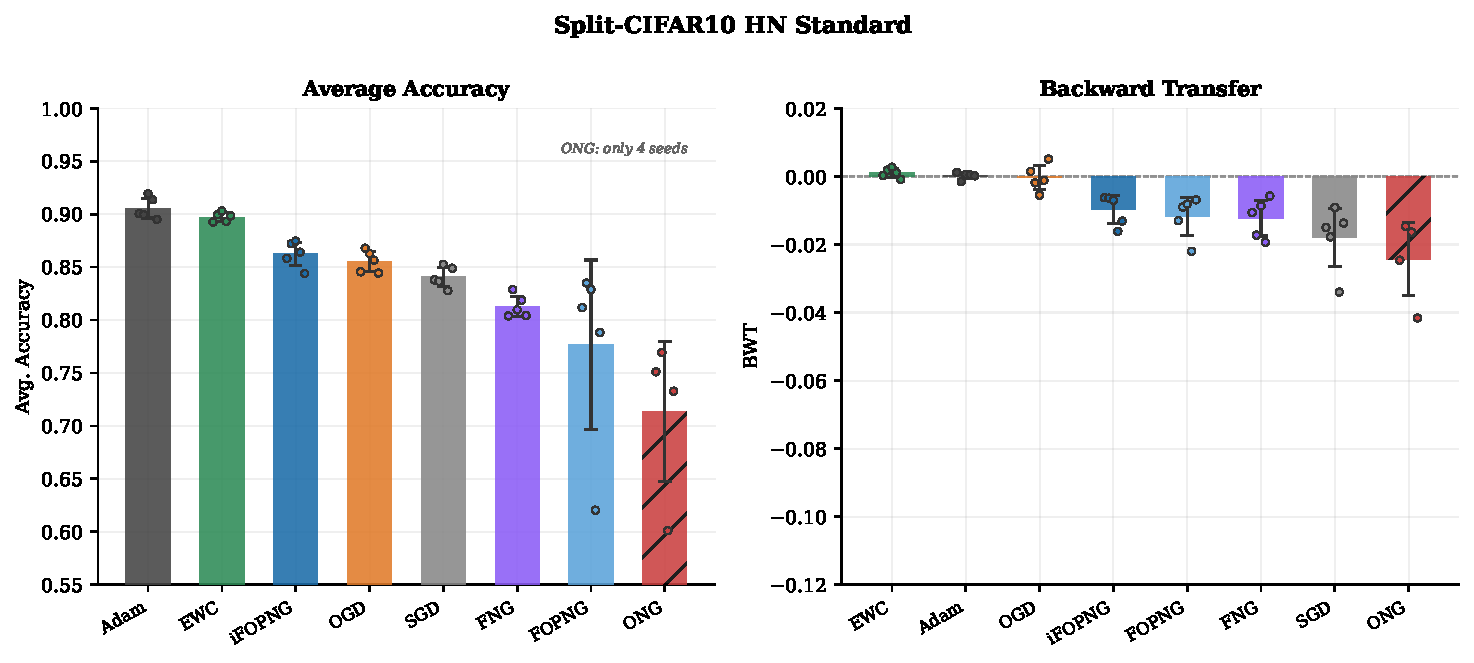
\includegraphics[width=\linewidth]{figures/hypernetwork-cifar10_8.pdf}
    \caption{%
        \textbf{Split-CIFAR10 hypernetwork (5 tasks, 50 epochs
        per task, AdamW first-task initialisation at $10^{-3}$).}
        Left: average accuracy (bars show mean over seeds; circles show
        individual seeds).
        Right: backward transfer. Methods are sorted by
        average accuracy on the left panel.
        \texttt{Adam} defines the projection-free upper frontier;
        \texttt{SGD} defines the unconstrained reference at $84.1\%$.
        \texttt{iFOPNG} is the only projection method to exceed \texttt{SGD};
        the remaining projection variants fall below it.
        All experiments use full normalization (Section~\ref{sec:results_rq2}).
    }
    \label{fig:hn_cifar10}
\end{figure}

\paragraph{Suffocated regime --- Split-MNIST, $d_h = 8$.}
Figure~\ref{fig:hn_suffocated} presents the full method comparison.
\texttt{Adam} leads at $92.7\%$.
\texttt{EWC} is the strongest regularization baseline at $87.5\%$, followed by the Fisher-free projection method \texttt{OGD} at $86.1\%$ and \texttt{SGD} at $78.4\%$.
The Fisher-based methods fall below: \texttt{iFOPNG} at $77.2\%$, \texttt{FOPNG} at $65.4\%$, and \texttt{FNG} at $63.4\%$.
Unlike previous observations, \texttt{iFOPNG}, \texttt{FOPNG}, and \texttt{FNG} all suffer from substantial negative backward transfer ($\mathrm{BWT}$ between $-0.15$ and $-0.21$), while \texttt{Adam} maintains a much smaller negative BWT ($-0.068$) and \texttt{SGD} forgets substantially ($-0.180$).

\begin{figure}[H]
    \centering
    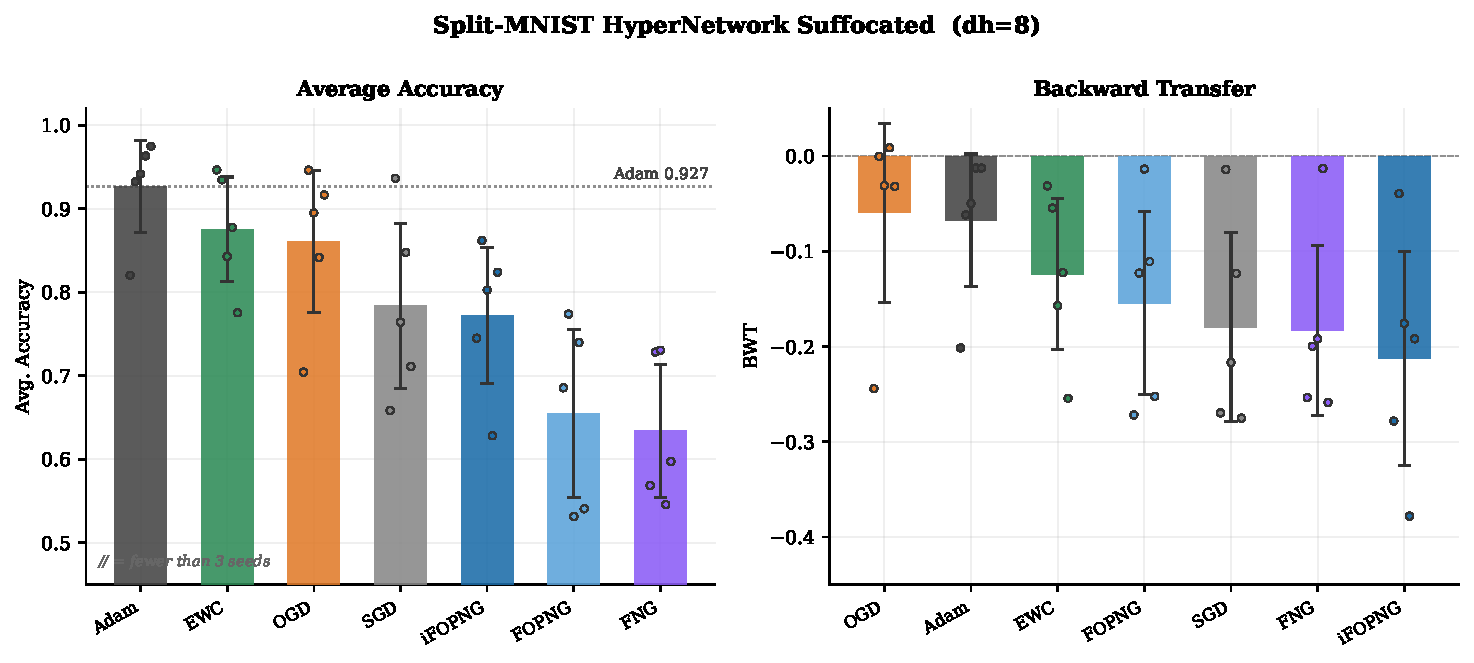
\includegraphics[width=\linewidth]{figures/hypernetwork-suffocated_7.pdf}
    \caption{%
        \textbf{Split-MNIST SH hypernetwork, suffocated
        regime ($d_h = 8$, 5 tasks, 15 epochs per task, \texttt{AdamW}
        first-task initialisation).}
        Left: average accuracy (bars show mean over seeds; circles show
        individual seeds).
        Right: backward transfer.
        The dotted line marks \texttt{Adam}'s mean accuracy ($92.7\%$).
        Fisher-based projection methods (\texttt{iFOPNG}, \texttt{FOPNG},
        \texttt{FNG}) suffer from significant negative BWT and lower accuracy than
        \texttt{Adam}, revealing a retention failure in the extreme compression regime.
        \texttt{EWC} is the best-performing baseline at $87.5\%$, while the Fisher-free \texttt{OGD} achieves $86.1\%$.
    }
    \label{fig:hn_suffocated}
\end{figure}

\paragraph{Extended task count --- Split-CIFAR100.}
At ten tasks on Split-CIFAR100 (Appendix~Figure~\ref{fig:hn_cifar100}), \texttt{EWC} unexpectedly leads at $45.5\%$, with \texttt{Adam} second at $42.0\%$ and \texttt{iFOPNG} third at $37.8\%$ (random baseline: $10.0\%$).

% ─────────────────────────────────────────────────────────────────────────────
\subsection{Sub-RQ2: Normalization Resolves the Gradient Pathology}
\label{sec:results_rq2}

This subsection reports the three-condition normalization ablation.
Figure~\ref{fig:norm_conditioning} traces the $\log_{10}$ condition number of the projection kernel $G^\top F G$ over training steps;
Figure~\ref{fig:norm_ablation} shows the resulting average accuracy and BWT under each condition.

\begin{figure}[H]
    \centering
    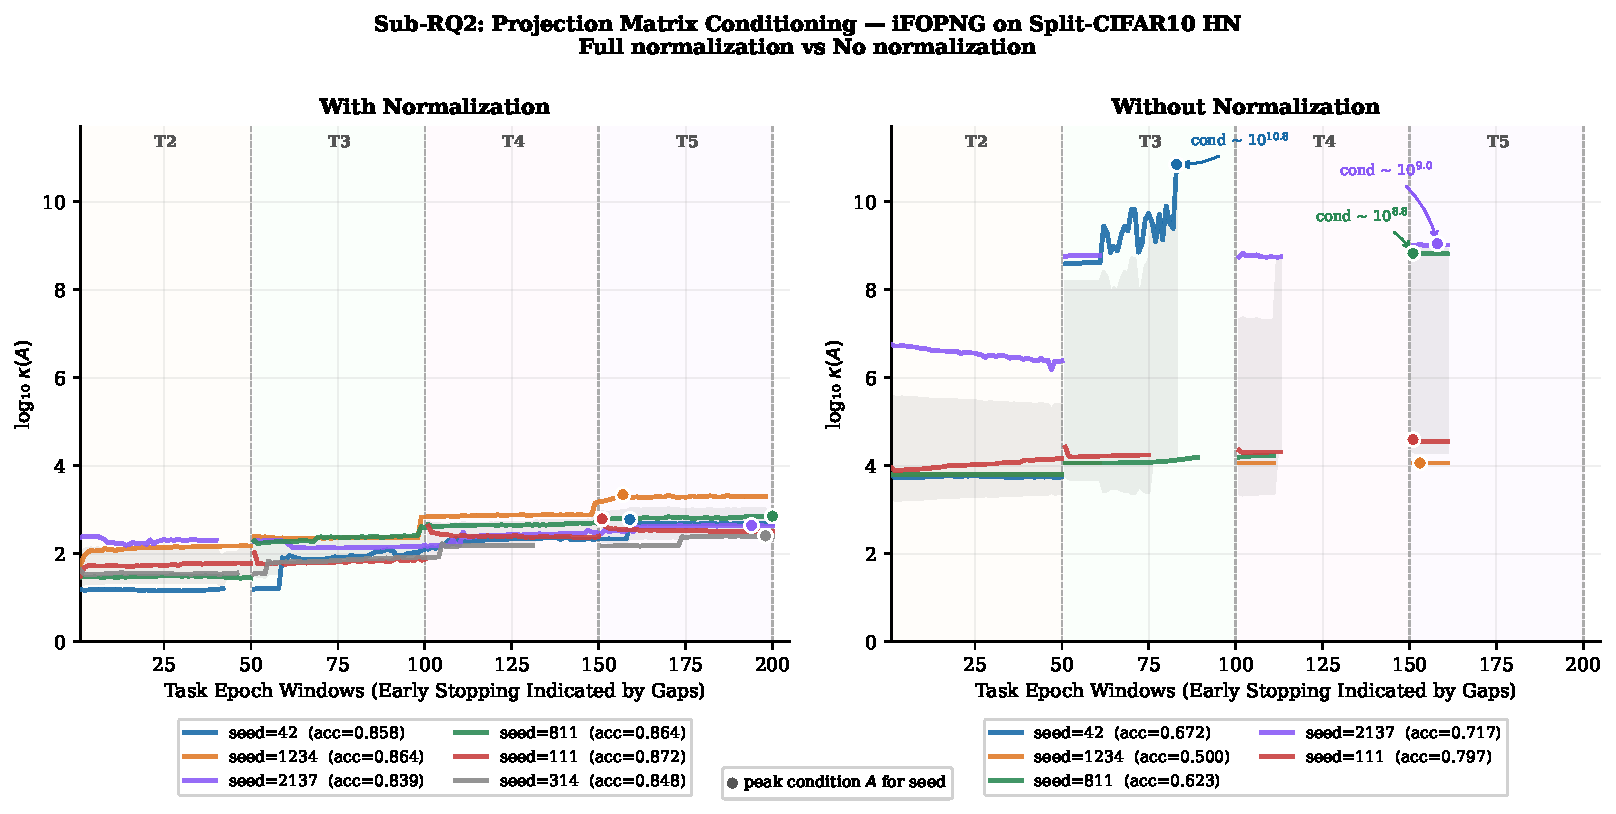
\includegraphics[width=\linewidth]{figures/normalization-conditioning_8-9.pdf}
    \caption{%
        \textbf{Projection kernel condition number over training ---
        \texttt{iFOPNG} on Split-CIFAR10 HN.}
        Each line is one seed (legend shows final average accuracy).
        Task boundaries are marked by vertical dashed lines; gaps indicate
        early stopping.
        Left (full normalization): $\log_{10}\kappa(A)$ remains bounded within $[10^{1.3},\,10^{3.3}]$ throughout.
        Right (no normalization): condition number spikes to
        $10^{10.8}$ at the T2$\to$T3 transition, causing projection failure.
        Diamond markers indicate end-of-task condition number values.
    }
    \label{fig:norm_conditioning}
\end{figure}

\begin{figure}[H]
    \centering
    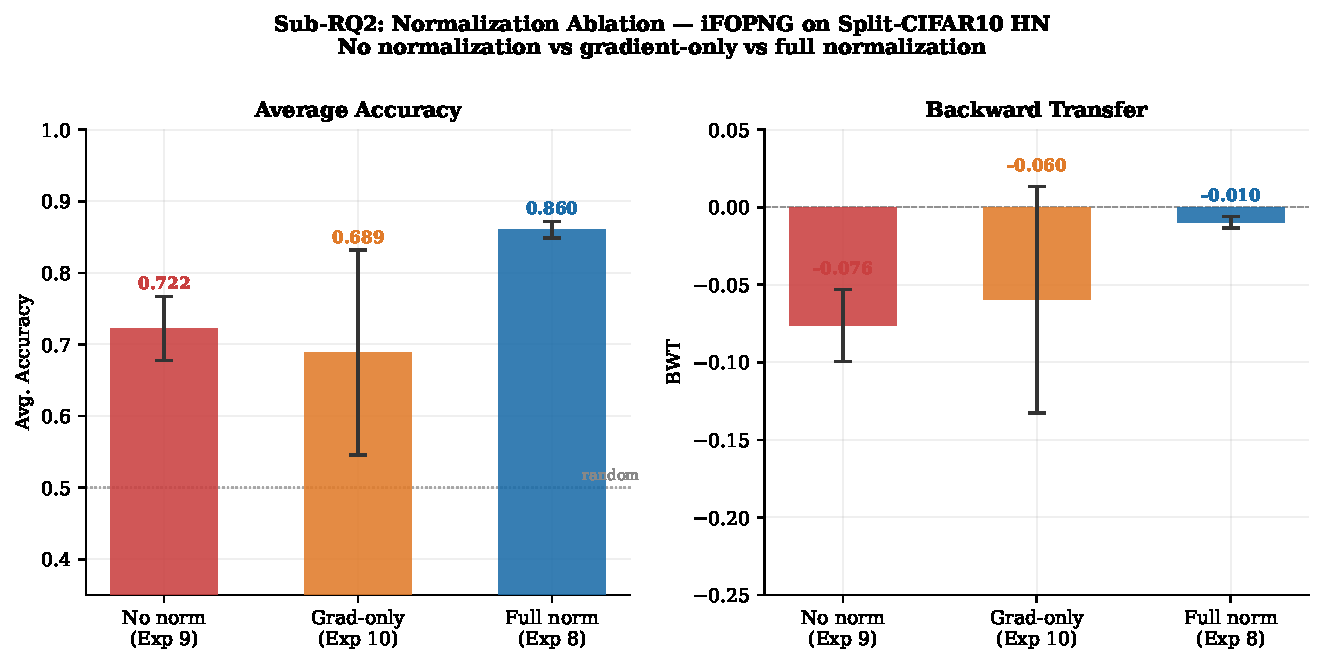
\includegraphics[width=0.75\linewidth]{figures/normalization-ablation_8-9-10.pdf} 
    \caption{%
        \textbf{Normalization ablation --- \texttt{iFOPNG} on Split-CIFAR10 HN
        (Sub-RQ2).}
        Three conditions: no normalization, gradient-only
        normalization, and full normalization.
        Left: average accuracy with mean annotated on each bar.
        Right: backward transfer.  Circles show individual seeds;
        bars show the mean.
        The dotted line on the left panel marks random-chance
        performance ($50\%$ for binary per-task classification).
    }
    \label{fig:norm_ablation}
\end{figure}

\paragraph{Without normalization.}
The right panel of Figure~\ref{fig:norm_conditioning} shows the condition number reaching $10^{10.8}$ at the T2$\to$T3 task transition for the most-affected seed, stabilizing near $10^{8.8}$--$10^{9.0}$ for two others.
The result is $72.2\%$ average accuracy and $\mathrm{BWT} = -0.076$.

\paragraph{Gradient-only normalization.}
Applying unit-$\ell_2$ column normalization to $G$ alone recovers $65.9\%$ (BWT $-0.065$), below both full normalization ($86.0\%$) and the no-normalization baseline ($72.2\%$) (Figure~\ref{fig:norm_ablation}).

\paragraph{Full normalization.}
Combining column-wise $\ell_2$ normalization of $G$ with absolute-maximum scaling of $F$ maintains $\log_{10}\kappa(A)$ bounded within $[10^{1.3},\,10^{3.3}]$ across all seeds and task transitions, a reduction of roughly seven orders of magnitude relative to the no-normalization condition (Figure~\ref{fig:norm_conditioning}).
Average accuracy recovers to $86.0\%$ and BWT improves to $-0.010$ (Figure~\ref{fig:norm_ablation}).

% ─────────────────────────────────────────────────────────────────────────────
\subsection{Sub-RQ3: Parameter Inertia via the Combined Fisher Metric}
\label{sec:results_rq3}

Figure~\ref{fig:ifopng_comparison} presents mean average accuracy for \texttt{iFOPNG} and \texttt{FOPNG} across all eight benchmarks.

\begin{figure}[H]
    \centering
    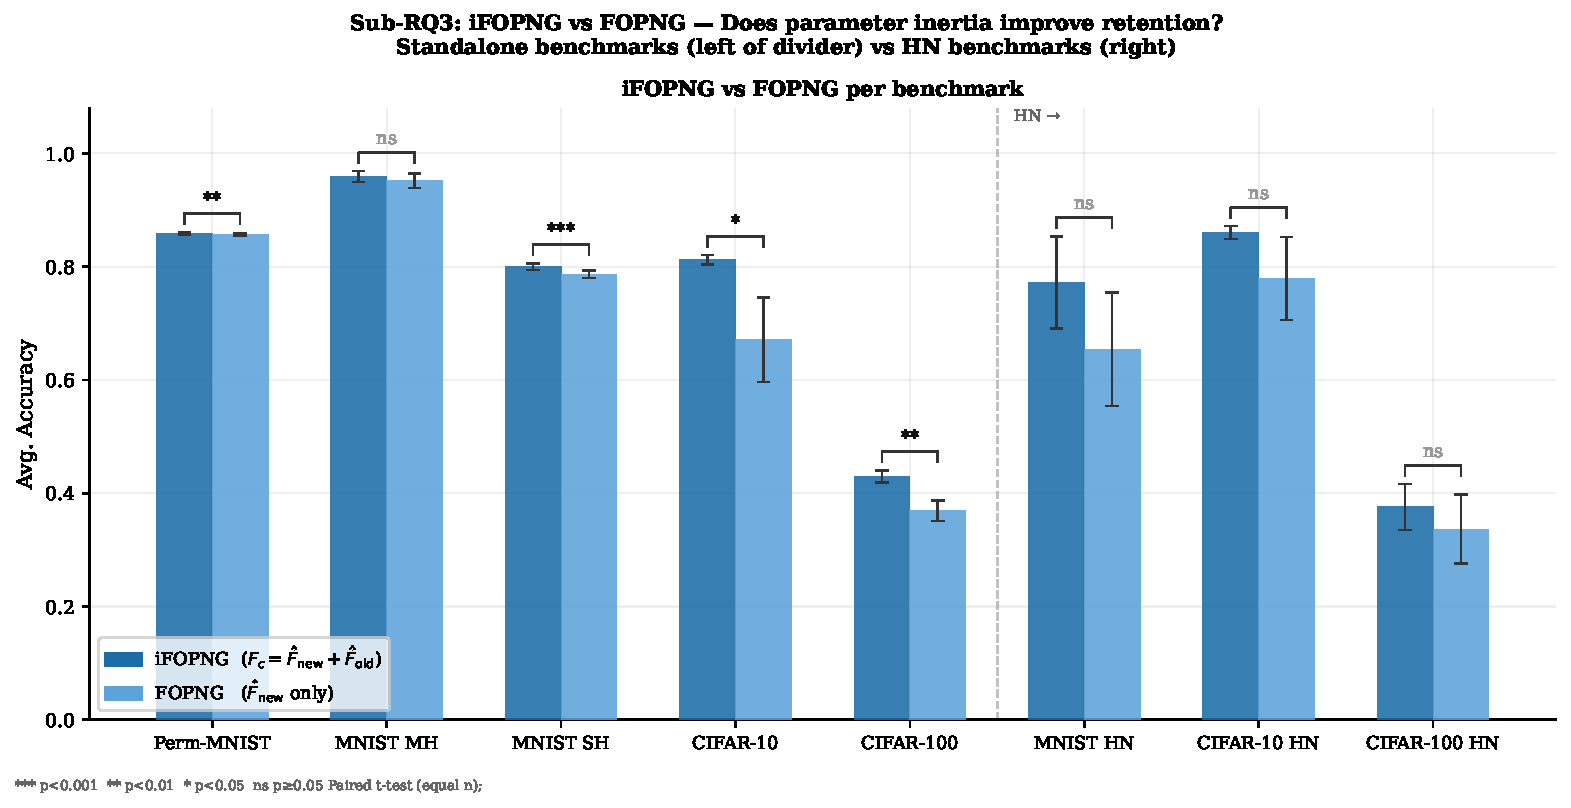
\includegraphics[width=\linewidth]{figures/projection-comparison_1-2-3-4-6-7-8.pdf}
    \caption{%
        \textbf{iFOPNG vs.\ FOPNG across eight benchmarks (Sub-RQ3).}
        Grouped bars show mean average accuracy;
        circles show individual seeds;
        error bars show $\pm 1$ standard deviation.
        The dashed vertical line
        separates standalone (left) from hypernetwork (right) settings.
        \texttt{iFOPNG} uses the combined metric
        $F_c = F_\mathrm{new} + F_\mathrm{old}$;
        \texttt{FOPNG} uses only $F_\mathrm{new}$.
    }
    \label{fig:ifopng_comparison}
\end{figure}

On the two simplest benchmarks the absolute differences are small, but the two cases 
diverge statistically. On Permuted-MNIST the $0.3$~pp advantage is negligible in size 
yet highly consistent across seeds, and reaches significance ($85.9\%$ vs.\ $85.7\%$, 
$t(4) = 6.38$, $p = .003$, $d_z = 2.85$, $n = 5$). On Split-MNIST multi-head a similarly 
small near-ceiling gap does not reach significance ($95.9\%$ vs.\ $95.2\%$, $t(4) = 1.12$, $p = .325$, $n = 5$).
% ─────────────────────────────────────────────────────────────────────────────
\subsection{Sub-RQ4: Fisher Accumulation Operator}
\label{sec:results_rq4}

This subsection compares two strategies for accumulating $F_\mathrm{old}$ across tasks under the \texttt{iFOPNG} combined Fisher metric: the element-wise maximum operator (MAX) and an exponential moving average (EMA).
Both are evaluated on a twenty-task Permuted-MNIST sequence with five random seeds.
Figure~\ref{fig:ema_trajectory} presents the average accuracy and backward transfer trajectories over all twenty tasks.

\begin{figure}[H]
    \centering
    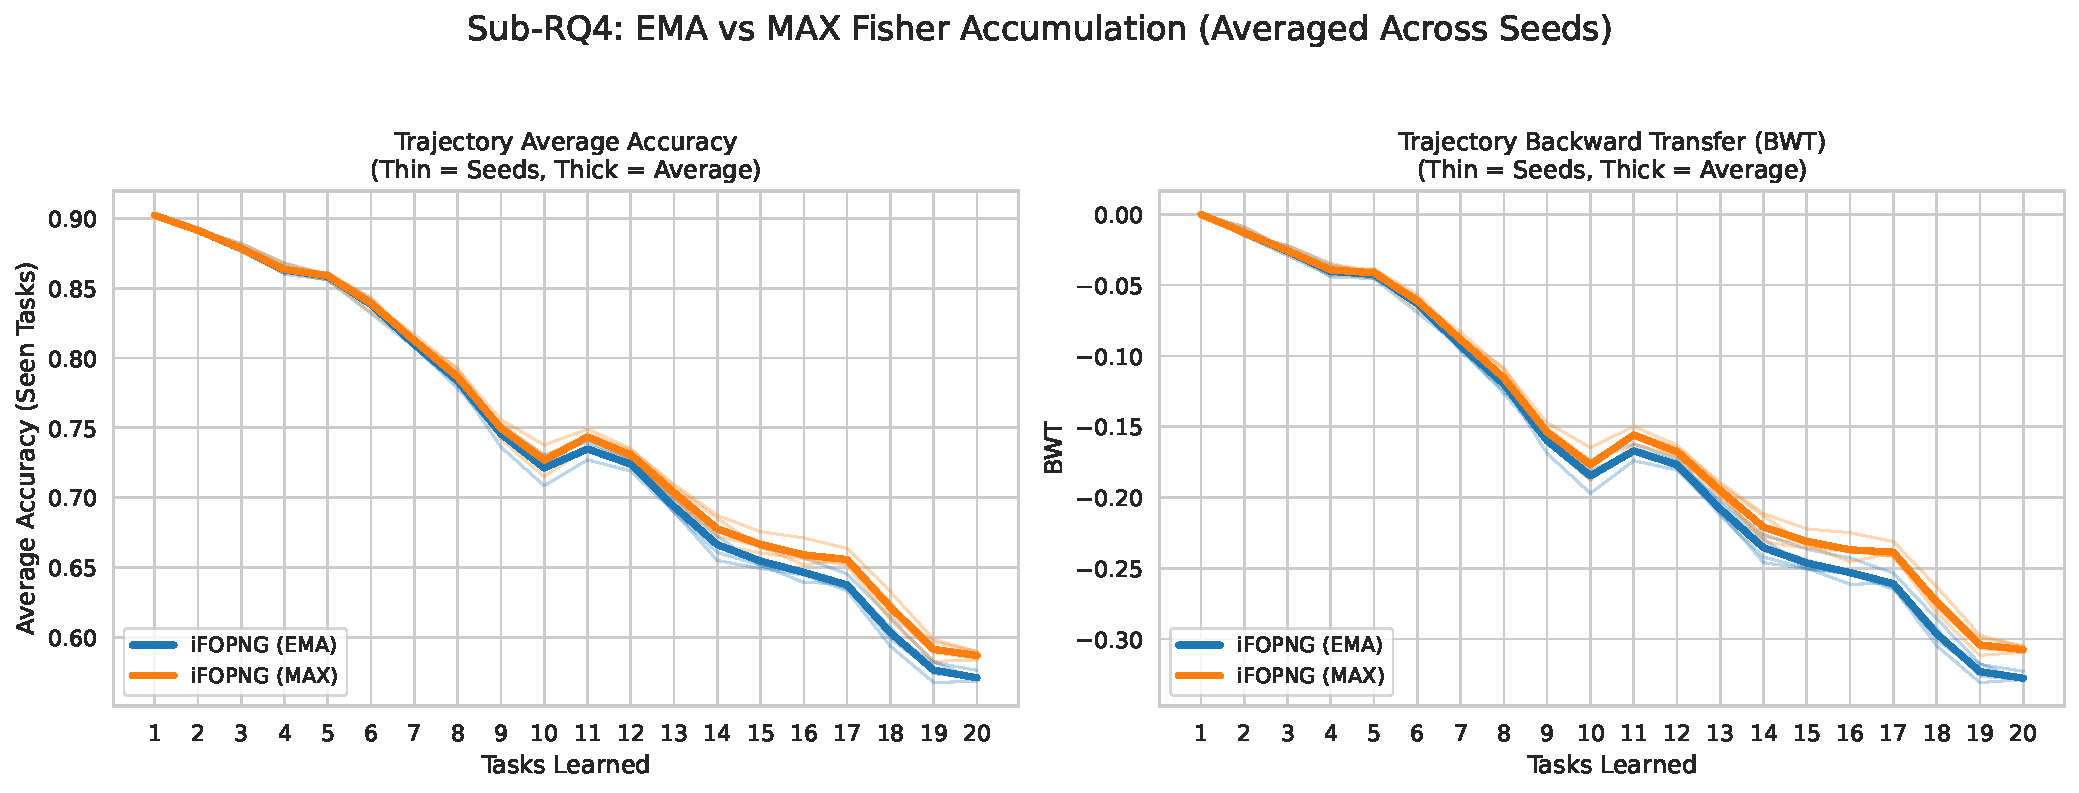
\includegraphics[width=\linewidth]{figures/ema-vs-max-trajectory_14-15.pdf}
    \caption{%
        \textbf{EMA vs.\ MAX Fisher accumulation trajectories on 20-task
        Permuted-MNIST (Sub-RQ4), $n = 5$ seeds.}
        Thick lines show the seed-averaged trajectory;
        thin lines show individual seeds.
        Left: average accuracy over tasks seen so far, evaluated after each
        task is trained.
        Right: backward transfer over the same sequence.
        MAX leads EMA by a consistent margin across all five seeds;
        both strategies produce closely tracking trajectories throughout the
        full twenty-task sequence.
    }
    \label{fig:ema_trajectory}
\end{figure}

A paired $t$-test on final average accuracy establishes MAX as the superior operator: $t(4) = 14.43$, $p < 0.001$, $d_z = 6.45$.
MAX leads EMA by $1.50$--$1.65$ percentage points across every seed pair without exception.

\section{Discussion}
\label{sec:discussion}
% Section 6.1 & 6.5: You handle this well currently. You refer to it simply as the "suffocated regime (dh​=8)"  without re-explaining the ablation. Leave these as they are
The overarching goal was to determine whether gradient projection methods
can be fruitfully integrated into chunked hypernetworks for continual
learning, and to identify the structural conditions under which this
integration succeeds or fails.

% ─────────────────────────────────────────────────────────────────────────────
\subsection{Sub-RQ1: Constructive Synergy or Architectural Conflict?}

Projection methods do not outperform a well-tuned regularized
hypernetwork optimized via \texttt{Adam}.
The gap of $4.5$~pp at task~5 in favor of \texttt{Adam} is consistent
across seeds and widens substantially in the suffocated regime ($d_h = 8$,
Split-MNIST SH), where it reaches $20$--$40$~pp.
Critically, the BWT data reveal that in the suffocated regime this is a
\emph{plasticity} failure, not a \emph{retention} failure: Fisher-based
projection methods achieve near-zero backward transfer alongside collapsed
accuracy, meaning the curvature-weighted constraint exhausts the available
gradient budget for new task learning rather than permitting forgetting of
prior ones.
\texttt{OGD}'s relative resilience at $d_h = 8$ is consistent with this
reading: without Fisher weighting its subspace constraint is less aggressive,
leaving more gradient capacity for forward transfer.
We attribute the broader gap to a fundamental architectural incompatibility.
Projection methods operate by modifying the raw gradient before the
optimizer state update, which means the first-order momentum estimate
and the adaptive scaling factor maintained by Adam are effectively
discarded at each projected step.
In the highly nonlinear, compressed weight space of a hypernetwork
meta-generator, momentum is not merely a convergence accelerant — it
is a structural regularizer that prevents the optimizer from committing
prematurely to poorly-conditioned gradient directions.
Re-initializing the optimizer's internal state at each step destabilizes
the generative manifold and reduces the quality of the generated weights,
particularly under extreme bottleneck compression.
This finding is consistent with \citet{hu_hidden_2026}, who demonstrate
that gradient modification methods interact adversely with Adam's internal
state under certain curvature regimes, and aligns with the broader
observation that projection-based continual learning methods were
originally designed for SGD-like updates.

The ten-task Split-CIFAR100 result introduces a partial rank reversal
that complicates the Sub-RQ1 conclusion: \texttt{EWC} unexpectedly leads
at $45.5\%$, overtaking both \texttt{Adam} ($42.0\%$) and \texttt{iFOPNG}
($37.8\%$).
As the number of tasks grows, the gradient subspace spanned by $G$ becomes
an increasingly coarse approximation to the full historical interference
manifold, while the functional regularizer grows more informative with each
additional stored weight snapshot.
Whether this effect persists at the twenty-task scale, and whether an
expanded memory budget would recover the projection advantage, remains to
be investigated.

\paragraph{First-task initialization and gradient contamination.}
Standard \texttt{Adam} couples weight decay into the gradient as an
additive $\ell_2$ term, so both $G$ and $\hat{F}$ collected at task~1
inherit a component aligned with weight magnitude rather than task loss
curvature, contaminating the projection subspace.
\texttt{AdamW}'s decoupled parameter-shrinkage step avoids this:
it consistently produced lower first-task trajectory variance and a
cleaner initial projection basis.
For any system bootstrapping a projection memory from first-task gradients,
the decoupled optimizer should be preferred at that stage.

% ─────────────────────────────────────────────────────────────────────────────
\subsection{Sub-RQ2: Projection-Scoped Normalization Resolves the Pathology}

The fundamental problem is purely numerical rather than conceptual:
the intersection of chunked hypernetworks and Fisher-weighted gradient
projection is geometrically coherent but arithmetically fragile without
explicit local rescaling.
This normalization is therefore a necessary engineering precondition for
any method that uses the Fisher metric within the projection algebra ---
specifically \texttt{FNG}, \texttt{FOPNG}, and \texttt{iFOPNG}.
\texttt{OGD}, which projects orthogonally without Fisher weighting,
maintains $G^\top G = I$ exactly through QR orthonormalization and is
structurally immune to the inversion collapse; its competitive performance
on the suffocated regime (Section~\ref{sec:results_rq1}) is consistent
with this immunity.
Severity scales with chunk count $C$ and training duration: gradient
magnitudes accumulate as $C \cdot g_\text{unit}$, Fisher as
$C^2 \cdot F_\text{unit}$, and the unnormalized projection matrix
inflates by order $C^4$ per task.
At sufficient scale the collapse is categorical rather than gradational
--- runs crash or converge to random-chance accuracy rather than merely
underperforming, as the elevated failure rate on the ten-task
Split-CIFAR100 hypernetwork illustrates even after normalization is applied
--- marking normalization as a structural stability prerequisite, not a
performance tuning.

% ─────────────────────────────────────────────────────────────────────────────
\subsection{Sub-RQ3: Parameter Inertia via the Combined Fisher Metric}
% LETS SAY HERE THAT HN RESULTS NEED TO BE TAKEN WITH A GRAIN OF SALT COMPARED TO REPLICATIONS OF GARG (STANDALONE RUNS).
\texttt{iFOPNG} outperforms \texttt{FOPNG} in all seven settings, confirming
that the combined metric $F_c = \hat{F}_\mathrm{new} + \hat{F}_\mathrm{old}$
yields consistent retention improvements.
The advantage is positive in every case and seed-consistent: even the
smallest gap, on Split-MNIST single-head ($+1.3$~pp), is statistically
unambiguous ($p < 0.001$, $d_z = 10.76$), indicating that the inertial
term reliably suppresses over-aggressive natural gradient steps at the
parameters that matter most to prior tasks whenever backbone and output-level
interference co-occur simultaneously.
The magnitude varies across benchmarks but the direction does not:
Sub-RQ3 is answered affirmatively.
\texttt{iFOPNG} does not close the gap to \texttt{Adam}, confirming that the
inertial combined metric improves retention by weighting historically important
coordinates more heavily, but cannot recover the adaptive momentum that
\texttt{Adam} leverages for efficient navigation of the generative manifold.

% ─────────────────────────────────────────────────────────────────────────────
\subsection{Sub-RQ4: Fisher Accumulation Operator}

On a twenty-task Permuted-MNIST sequence, the
element-wise maximum (MAX) accumulation strategy
systematically outperformed the exponential
moving average (EMA).
While the $1.60$~pp advantage is small,
it is statistically unambiguous ($p < 0.001$).
Crucially, the hypothesized plasticity cost
of MAX's monotonic growth did not materialize.
Because our normalization scheme rescales
both Fisher terms, the projection becomes
insensitive to absolute scale, relying
solely on relative parameter distributions.
Therefore, MAX remains the definitive practical choice:
it is simpler, hyperparameter-free, and
marginally superior, though highly heterogeneous
task distributions could potentially introduce divergence.

% ─────────────────────────────────────────────────────────────────────────────
\subsection{Limitations}

Several limitations should be acknowledged.

First, the hypernetwork results presented here are restricted to
Split-MNIST and Split-CIFAR10 with five tasks.
Longer task sequences may produce different relative orderings:
in particular, the advantage of hard projection constraints over soft
functional regularization may grow with sequence length, as soft
penalties are known to suffer from compounding output drift
\citep{farquhar_towards_2018}, while the projection subspace scales with
the gradient budget rather than the task count.
The preliminary ten-task Split-CIFAR100 result, in which EWC overtakes both
\texttt{Adam} and \texttt{iFOPNG}, is suggestive but insufficient to
establish a trend; a systematic sweep over task count is warranted.

Second, the results are specific to the constrained-capacity regimes
examined here.
For Split-MNIST, a standard-capacity hypernetwork solves the benchmark
near-trivially regardless of the continual learning method applied;
the suffocated setting ($d_h = 8$) is deliberately chosen to place the
architecture below saturation, where method differences are measurable.
For Split-CIFAR10, the convolutional target network is large enough that
the hypernetwork already operates under a natural capacity constraint,
and meaningful method separation emerges without artificial bottlenecking.
Whether the projection--hypernetwork interaction studied here generalises
to harder benchmarks requiring larger target architectures --- where the
hypernetwork must generate weights for deeper convolutional or
attention-based networks and the task itself is sufficiently complex to
prevent ceiling effects --- remains an open question.
In such settings, the gradient accumulation pathology documented here
would be substantially more severe: chunk counts scale with the target
parameter count, so the condition number blowup $\sim C^4$ identified
here represents a lower bound on the numerical challenge at scale.

Third, the proposed normalization scheme---QR orthonormalization combined with
absolute-maximum Fisher scaling---is fundamentally heuristic in nature. While it
successfully eliminates the numerical pathology of condition number collapse,
it applies isotropic rescaling to the projection basis. This likely discards
important geometric properties of the Fisher metric, temporarily divorcing the
subspace constraint from the true curvature of the parameter space.
A mathematically principled formulation that stabilizes the projection algebra
while strictly preserving the theoretical guarantees of Fisher-based methods
remains an open question for future work.

% WRONG This thesis didnt validate to what extent can gradient projection methods be
% implemented for hypernetworks. THAT WAS THE FIRST PREMISE. But I failed to create a
% principled normalization structure for this combination. 

% NOW the rq1 looks like this:
% \item[\textbf{Sub-RQ1}] \textbf{(Synergy vs.\ Conflict):} Does the joint
% integration of hard gradient projection with the hypernetwork's soft
% functional regularizer yield a constructive
% synergy, or does a standalone regularized hypernetwork offer a more
% efficient optimization frontier?

% So basically I didnt resolve that question. I made one attempt but it basically failed
% to improve the performance of hypernetworks as plain adam with hypernetwork outperformed every 
% other method

\section{Conclusion}
\label{sec:conclusion}

This thesis investigated integrating gradient projection
methods into chunked hypernetworks for continual learning.
We primarily diagnosed the architectural boundaries
and numerical pathologies governing this core integration.
Alongside these fundamental structural findings, we
also evaluated adjacent methodological optimizations regarding
parameter inertia and Fisher matrix accumulation.

\paragraph{Sub-RQ1 --- Partial Synergy and the Momentum Bottleneck.}
The synergy between hard gradient projection and
soft functional regularization is constructive but bounded.
While \texttt{iFOPNG} outperforms unconstrained \texttt{SGD}
in standard-capacity settings, standalone regularized
hypernetworks optimized via \texttt{Adam} remain
vastly superior.

This performance gap stems from an architectural
conflict, not projection geometry.
Under extreme compression ($d_h = 8$), Fisher-based
projection methods suffer a severe \emph{retention}
failure, experiencing substantial negative backward transfer
as the constraint fails to protect prior knowledge.
Because projection modifies raw gradients before the
optimizer updates, it discards adaptive momentum.
In hypernetworks, this momentum acts as a crucial
structural regularizer; without it, the network commits
prematurely to poorly-conditioned gradient directions,
destabilizing the generative manifold and causing
catastrophic interference.

Ultimately, the loss of adaptive momentum is
the binding constraint.
Integrating gradient projection into hypernetworks
will require projection-compatible adaptive optimizers,
rather than post-hoc gradient modifications \citep{hu_hidden_2026}.

\paragraph{Sub-RQ2 --- Normalization Is a Necessary Condition.}
Without explicit local rescaling, projection methods are numerically
incompatible with chunked hypernetworks: matrix inversion in the
projection kernel degrades or collapses entirely depending on chunk
count, pulling performance below plain SGD.
QR orthonormalization of the gradient basis combined with
absolute-maximum Fisher scaling resolves the pathology in the tested
configurations.
This normalization scheme is a necessary engineering precondition for
any future combination of gradient projection with chunked
meta-learners, regardless of which projection algebra is employed.

\paragraph{Sub-RQ3 --- Parameter Inertia via Combined Fisher Metric.}
Replacing the task-specific Fisher metric with the combined inertial metric
($F_c$) improves retention in direction across every benchmark tested.
The advantage is statistically significant on four of the five standalone
benchmarks, including Permuted-MNIST, where it is negligible in size
($+0.3$~pp) yet reliable on account of its consistency across seeds; the only
standalone null is the near-ceiling Split-MNIST multi-head ($+0.7$~pp,
$p = .325$). The advantage is largest on Split-CIFAR10 ($+14.1$~pp,
$p = .024$), alongside a substantial gain on Split-MNIST single-head ($+1.3$~pp). 
The same positive direction carries into the three hypernetwork
settings, though none reaches significance under the elevated inter-seed
variance of that regime. Integrating parameter inertia therefore yields a
positive retention advantage in every setting: statistically robust across the
standalone benchmarks, and directionally consistent but underpowered in the
hypernetwork settings.

\paragraph{Sub-RQ4 --- MAX Accumulation Is the Clear Practical Choice.}
On a twenty-task sequence the element-wise maximum operator was statistically
superior to an exponential moving average (${\sim}1.60$~pp, $p < 0.001$),
and the hypothesised plasticity cost of its monotonic growth did not
materialise. MAX is therefore preferred: hyperparameter-free, simpler, and
marginally better.

\paragraph{Implications for the field.}
The results establish a clear empirical boundary for the current generation
of gradient projection methods: they can be made numerically stable in
chunked hypernetwork settings via local rescaling, and their Fisher geometry
can be improved via the combined Fisher metric $F_c$, but the momentum incompatibility
prevents them from reaching the performance frontier of adaptive
unconstrained optimizers in generative parameter spaces.
The normalization contribution is directly applicable to any method that
maintains a gradient subspace memory alongside a chunked weight generator.
The iFOPNG contribution extends naturally to any continual learning
setting where Fisher overlap accumulates across tasks.
Together, they narrow the gap between projection-based and
regularization-based approaches, and provide a principled foundation for
the next step: a projected adaptive optimizer that respects both the
geometric constraints of the projection and the curvature structure that
adaptive moment estimates capture.



\section*{Acknowledgements}
The author thanks dr.\ Giacomo Spiegler for supervision and valuable feedback throughout this project.
\newpage
\bibliography{references}

\clearpage
\section{Appendix}
\section*{Appendix A: iFOPNG Theorem and Proof}
\label{app:a}

% ─────────────────────────────────────────────────────────────────────────────
% PREAMBLE REQUIREMENT: this appendix uses the environments
%   assumption, theorem, lemma, proposition, corollary, remark.
% If any are missing from the preamble, add (after \usepackage{amsthm}):
%   \newtheorem{lemma}{Lemma}
%   \newtheorem{proposition}{Proposition}
%   \newtheorem{corollary}{Corollary}
%   \theoremstyle{remark}\newtheorem{remark}{Remark}
% ─────────────────────────────────────────────────────────────────────────────

\subsection*{Notation}

Throughout this proof, $g \in \mathbb{R}^p$ denotes the current gradient,
$G \in \mathbb{R}^{p \times m}$ the memory matrix of $m$ historical gradient
directions (each orthonormalised at insertion via QR; the proof does not
rely on this property), and $F_{\mathrm{new}}$, $F_{\mathrm{old}}$ the
current-task and accumulated diagonal empirical Fisher tensors, with
$F_c = F_{\mathrm{new}} + F_{\mathrm{old}}$.
Diagonal Fisher tensors are treated as vectors acting by element-wise
multiplication and are identified with the corresponding diagonal matrices,
which are symmetric.
For a symmetric positive-definite $S$ we write $\|w\|_S = \sqrt{w^\top S w}$.
The projection kernel is
\begin{equation}
    A \coloneqq G^\top F_{\mathrm{old}}\, F_c^{-1}\, F_{\mathrm{old}}\, G
    \;\in\; \mathbb{R}^{m \times m}.
\end{equation}

\begin{assumption}[Regularity]
\label{ass:regularity}
$F_c$ is positive definite and the kernel $A$ is invertible.
\end{assumption}

\noindent
Both conditions hold unconditionally in the implementation, which inverts the
damped matrices $F_c + \hat\lambda I$ and $A + \hat\lambda I$ with
$\hat\lambda > 0$ (Section~\ref{sec:normalization}); the theorem below states
the exact $\lambda \to 0$ result.

\begin{theorem}[iFOPNG Update]
\label{thm:ifopng}
Under Assumption~\ref{ass:regularity}, the solution to
\begin{equation}
\label{eq:ifopng_problem}
\begin{aligned}
    \min_{u}\;\; & \bigl\| g - F_c^{-1} u \bigr\|_{F_c}^2 \\
    \mathrm{s.t.}\;\; & F_{\mathrm{old}}^{-1} u \in \operatorname{Col}(G), \\
                       & \|v\|_{F_c} = \eta,
\end{aligned}
\end{equation}
with parameter update $v = \gamma\, F_c^{-1}(g - u)$, is given by
Equation~\eqref{eq:ifopng}:
\begin{equation}
    v^* = -\eta\,
    \frac{F_c^{-1} P g}{\sqrt{(Pg)^\top F_c^{-1} P g}},
    \qquad
    P = I - F_{\mathrm{old}}\, G\, A^{-1}\, G^\top F_{\mathrm{old}}.
\end{equation}
\end{theorem}

\begin{proof}
\textbf{Step 1 (parameterise the constraint).}
The constraint $F_{\mathrm{old}}^{-1} u \in \operatorname{Col}(G)$ means
$F_{\mathrm{old}}^{-1} u = G\alpha$ for some $\alpha \in \mathbb{R}^m$,
i.e.\ $u = F_{\mathrm{old}}\, G\, \alpha$.
The optimisation over the constrained $u$ thus reduces to an unconstrained
optimisation over $\alpha \in \mathbb{R}^m$.

\textbf{Step 2 (expand the objective).}
Writing $\|w\|_{F_c}^2 = w^\top F_c\, w$ and using $F_c^{-1} F_c = I$,
\begin{equation}
    \bigl\| g - F_c^{-1} u \bigr\|_{F_c}^2
    = g^\top F_c\, g \;-\; 2\, g^\top u \;+\; u^\top F_c^{-1} u .
\end{equation}
Substituting $u = F_{\mathrm{old}}\, G\, \alpha$, the linear term becomes
$-2\,(G^\top F_{\mathrm{old}}\, g)^\top \alpha$ and the quadratic term
becomes $\alpha^\top A\, \alpha$, since
$G^\top F_{\mathrm{old}}\, F_c^{-1}\, F_{\mathrm{old}}\, G = A$.
The first term $g^\top F_c\, g$ does not depend on $\alpha$.

\textbf{Step 3 (minimise).}
The reduced objective is quadratic in $\alpha$ with Hessian $2A \succ 0$,
hence strictly convex.
Setting its gradient to zero gives the normal equations
$A\,\alpha^* = G^\top F_{\mathrm{old}}\, g$, with unique solution
\begin{equation}
\label{eq:alpha_star}
    \alpha^* = A^{-1}\, G^\top F_{\mathrm{old}}\, g .
\end{equation}

\textbf{Step 4 (back-substitute).}
Inserting $\alpha^*$ into $u = F_{\mathrm{old}}\, G\, \alpha$ gives
$u^* = F_{\mathrm{old}}\, G\, A^{-1}\, G^\top F_{\mathrm{old}}\, g$, so
\begin{equation}
    g - u^* = \bigl(I - F_{\mathrm{old}}\, G\, A^{-1}\,
              G^\top F_{\mathrm{old}}\bigr) g = P g .
\end{equation}

\textbf{Step 5 (apply the trust region).}
For $v = \gamma\, F_c^{-1} P g$,
\begin{equation}
    \|v\|_{F_c}^2
    = \gamma^2\,(Pg)^\top F_c^{-1} F_c\, F_c^{-1} (Pg)
    = \gamma^2\,(Pg)^\top F_c^{-1} (Pg).
\end{equation}
Imposing $\|v\|_{F_c} = \eta$ fixes
$|\gamma| = \eta / \sqrt{(Pg)^\top F_c^{-1} P g}$.
The negative root is selected so that with empty memory ($P = I$) the update
reduces to the natural-gradient descent step under $F_c$, matching the
\texttt{FOPNG} convention \citep{garg_fisher-orthogonal_2026}.
This yields the stated update:
\begin{equation}
    v^* = -\eta\, \frac{F_c^{-1} P g}{\sqrt{(Pg)^\top F_c^{-1} P g}}.
\end{equation}
\end{proof}

\begin{remark}[Relationship to FOPNG]
The single substitution $F_{\mathrm{new}} \to F_c$ recovers \texttt{FOPNG}:
the proof is identical with $F_c$ replaced by $F_{\mathrm{new}}$ in the
metric, the kernel $A$, and the trust region.
\texttt{iFOPNG} differs only in that the ambient metric carries the
accumulated historical curvature $F_{\mathrm{old}}$ in addition to the
current-task curvature.
\end{remark}

\begin{remark}[Inertia mechanism]
The trust-region budget splits additively across the two geometries:
\begin{equation}
    \|v\|_{F_c}^2
    = v^\top F_{\mathrm{new}}\, v + v^\top F_{\mathrm{old}}\, v
    = \|v\|_{F_{\mathrm{new}}}^2 + \|v\|_{F_{\mathrm{old}}}^2 = \eta^2 .
\end{equation}
A coordinate with large $(F_{\mathrm{old}})_i$ consumes more of the shared
budget $\eta^2$ per unit of motion and is therefore moved less.
This is the sense in which historical importance acts as inertia rather than
as a restoring force: no reference point and no penalty term enter the
objective, in contrast to EWC \citep{kirkpatrick_overcoming_2017}.
\end{remark}

\subsection*{Algorithm Statements}

Algorithm~\ref{alg:prefisher} is reproduced from
\citet{garg_fisher-orthogonal_2026} without modification.
It pre-multiplies each stored gradient by the Fisher estimate of the task it
was collected on, absorbing the metric weighting into $\tilde{G}$ at
collection time so that $\tilde{G}$ approximates $F_{\mathrm{old}}\,G$ (up to
subsequent element-wise maximum updates of $F_{\mathrm{old}}$) and the
per-iteration projection reduces to a single matrix--vector product against
$\tilde{G}$.
Empirically the two algorithms produce indistinguishable results on all
benchmarks evaluated here; \texttt{preIFOPNG} is the implementation preferred
in practice due to its reduced cost.

% ── Algorithm 1: iFOPNG ──────────────────────────────────────────────────────

\begin{algorithm}[htbp]
\caption{iFOPNG Algorithm (extends \texttt{FOPNG}~\citep{garg_fisher-orthogonal_2026}
       via combined metric $F_c$)}
\label{alg:ifopng}
\small
\setlength{\abovedisplayskip}{2pt}
\setlength{\belowdisplayskip}{2pt}
\begin{algorithmic}[1]
\Require Initial parameters $\theta_0$, task sequence $\{D_1,\ldots,D_T\}$,
              learning rate $\eta$, damping $\lambda$,
              number of stored gradients per task $k$, number of epochs $E$
\State Initialize gradient memory $G \leftarrow [\,]$.
       Train on task $D_1$ using Adam or SGD.
\State Compute $F_{\mathrm{old}} \leftarrow F(D_1)$;\quad
       Store $G \leftarrow [g_1, \ldots, g_k]$
\For{task $t = 2, 3, \ldots, T$}
       \For{epoch $e = 1, \ldots, E$}
              \State Recompute new-task Fisher:
                     ${F}_{\mathrm{new}} \leftarrow F(D_t)$;
              \State Form combined metric:
                     $F_c \leftarrow F_{\mathrm{new}} + F_{\mathrm{old}}$
              \For{all batches $(x, y)$ in $D_t$}
              \State Compute gradient $g \leftarrow \nabla_\theta \mathcal{L}_t(\theta)$
              \State Compute $v^*$ according to Theorem~\ref{thm:ifopng}
                     under metric $F_c$
              \State Update parameters: $\theta \leftarrow \theta + v^*$
              \EndFor
       \EndFor
       \State Store gradients:
              $G \leftarrow [G,\; g_{k(t-1)+1}, \ldots, g_{kt}]$
       \State Update accumulated Fisher:
              $F_{\mathrm{old}} \leftarrow
              \max\!\left(F_{\mathrm{old}},\, F_{\mathrm{new}}\right)$
\EndFor
\end{algorithmic}
\end{algorithm}

% ── Algorithm 2: preIFOPNG ───────────────────────────────

\begin{algorithm}[htbp]
\caption{preIFOPNG Algorithm~\citep{garg_fisher-orthogonal_2026},
       adapted for the iFOPNG combined metric}
\label{alg:prefisher}
\small
\setlength{\abovedisplayskip}{2pt}
\setlength{\belowdisplayskip}{2pt}
\begin{algorithmic}[1]
\Require Initial parameters $\theta_0$, task sequence $\{D_1,\ldots,D_T\}$,
              learning rate $\eta$, damping $\lambda$,
              number of stored gradients per task $k$, number of epochs $E$
\State Initialize pre-Fisher memory $\tilde{G} \leftarrow [\,]$.
       Train on task $D_1$ using Adam or SGD.
\State Compute $F_1 \leftarrow F(D_1)$;\quad
       $F_{\mathrm{old}} \leftarrow F_1$;\quad
       Store $\tilde{G} \leftarrow [F_1 \odot g_1, \ldots, F_1 \odot g_k]$
\For{task $t = 2, 3, \ldots, T$}
       \For{epoch $e = 1, \ldots, E$}
              \State Recompute new-task Fisher:
                     $F_{\mathrm{new}} \leftarrow F(D_t)$;
              \State Form combined metric:
                     $F_c \leftarrow F_{\mathrm{new}} + F_{\mathrm{old}}$
              \For{all batches $(x, y)$ in $D_t$}
              \State Compute gradient $g \leftarrow \nabla_\theta \mathcal{L}_t(\theta)$
              \State Compute $v^*$ according to Theorem~\ref{thm:ifopng}
                     using $\tilde{G}$ in place of $G$
              \State Update parameters: $\theta \leftarrow \theta + v^*$
              \EndFor
       \EndFor
       \State Compute $F_t \leftarrow F(D_t)$;\quad
              Store $\tilde{G} \leftarrow
              [\tilde{G},\; F_t \odot g_{k(t-1)+1},
              \ldots, F_t \odot g_{kt}]$
       \State Update accumulated Fisher:
              $F_{\mathrm{old}} \leftarrow
              \max\!\left(F_{\mathrm{old}},\, F_{\mathrm{new}}\right)$
\EndFor
\end{algorithmic}
\end{algorithm} % A

% ─────────────────────────────────────────────────────────────────────────────
% Appendix B: Standalone Target-Network Results
% ─────────────────────────────────────────────────────────────────────────────
\section*{Appendix B: Standalone Target-Network Results}
\label{app:standalone}
This appendix presents the full method comparison on standalone target
networks --- configurations where a conventional MLP is trained directly via
gradient projection, without any hypernetwork wrapper or functional
regulariser. These results establish the baseline behaviour of each projection
method in its intended setting, prior to the hypernetwork integration examined
in the main text. All five benchmark streams are reported as per-task accuracy
trajectories in a single figure (Figure~\ref{fig:standalone_trajectories_all}):
Permuted-MNIST (5 tasks), Split-MNIST single-head (5 tasks), Split-MNIST
multi-head (5 tasks), Split-CIFAR10 (5 tasks), and Split-CIFAR100 (10 tasks).

% ── B.1  All benchmarks, single figure TRAJECTORIES ──────────────────────────
\begin{figure}[H]
    \centering
    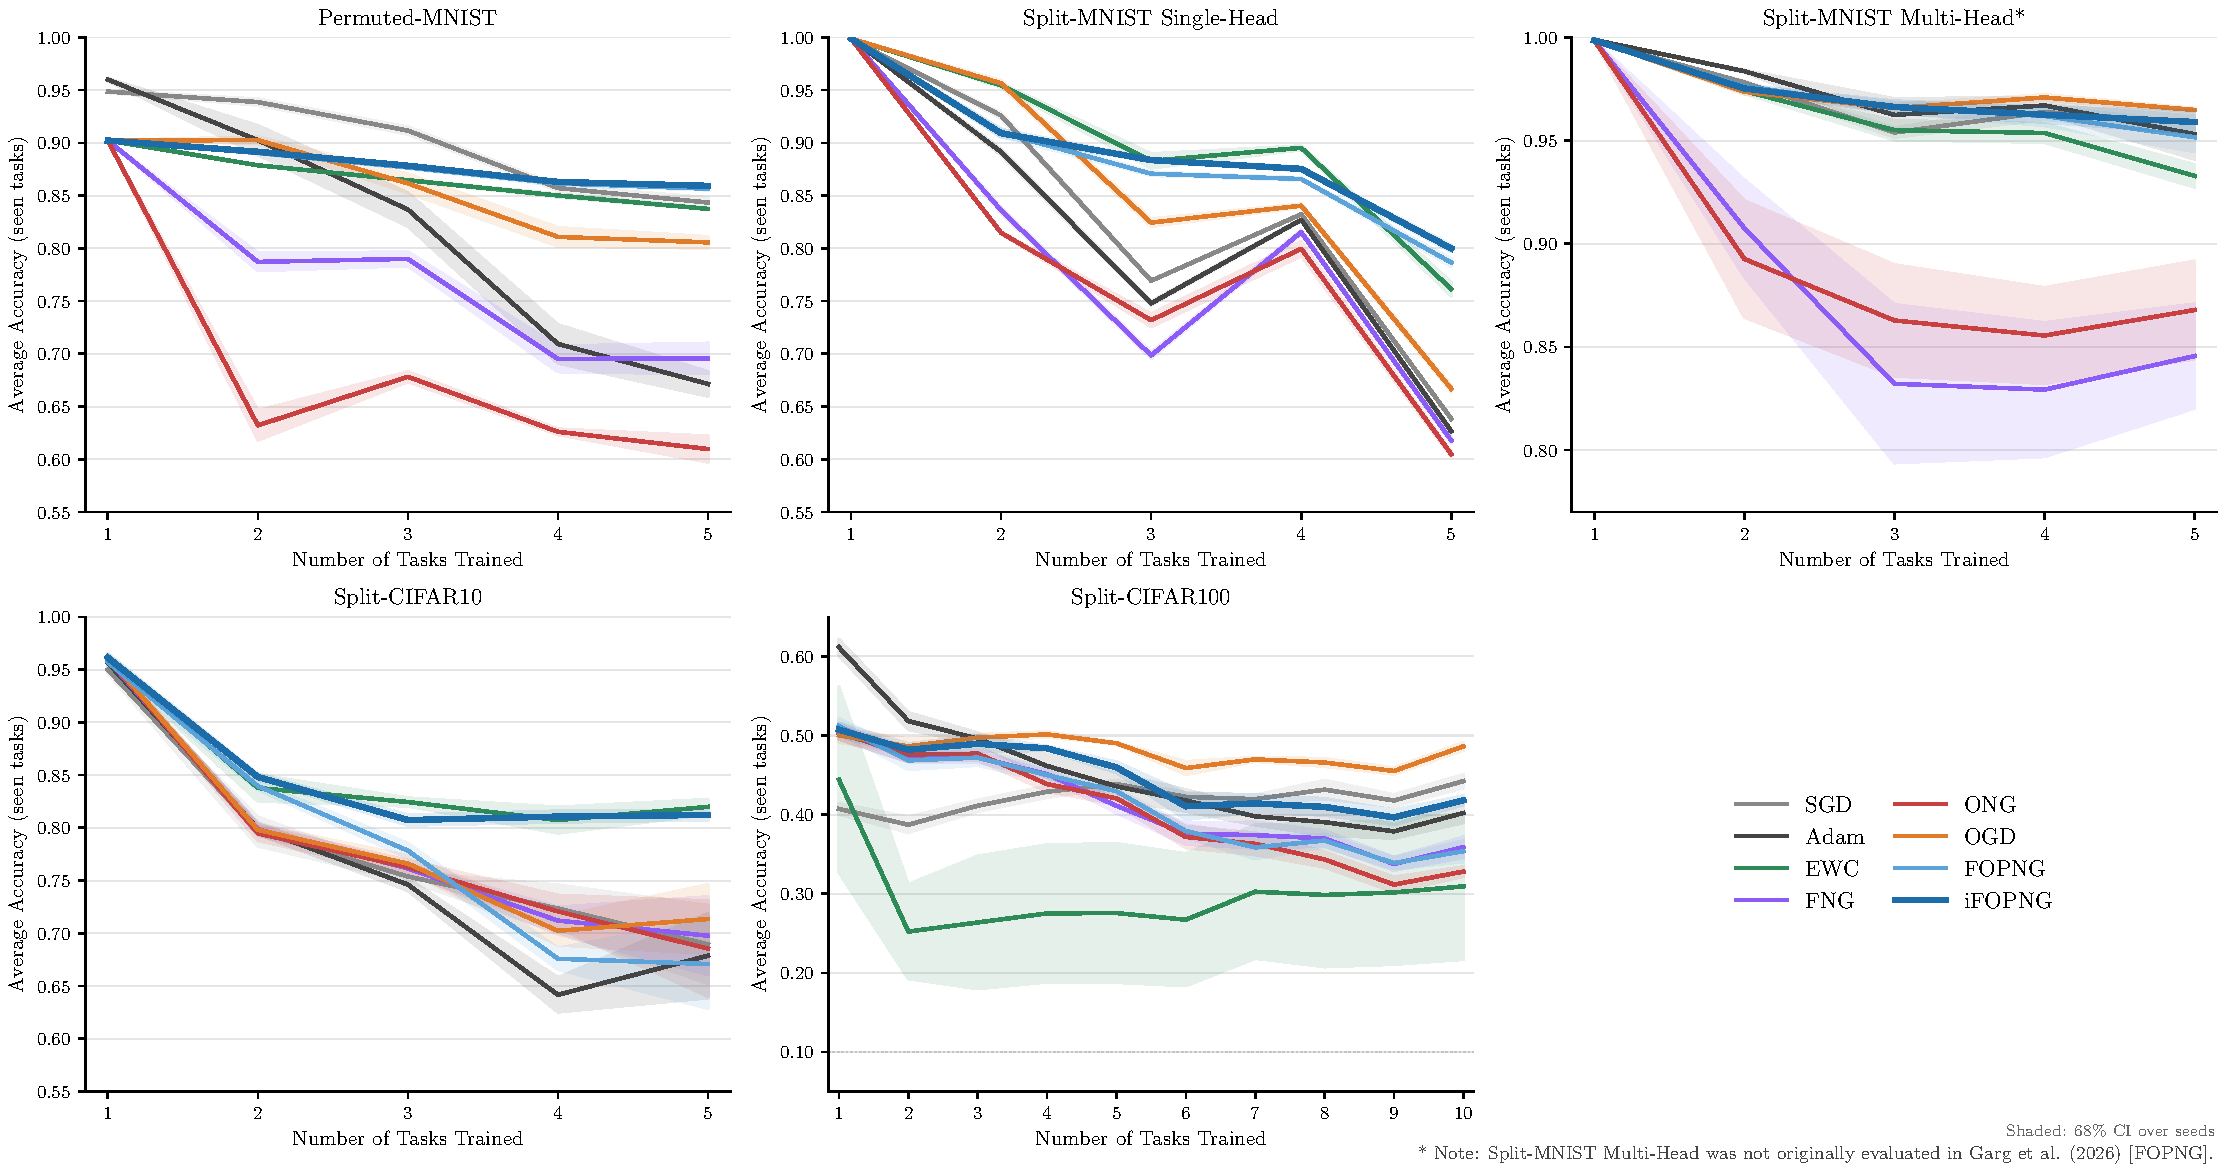
\includegraphics[width=\linewidth,height=0.82\textheight,keepaspectratio]{figures/garg-repl-grid.pdf}
    \caption{%
        \textbf{Standalone target-network accuracy trajectories across all
        benchmarks, replicating the evaluation protocol of
        \citet{garg_fisher-orthogonal_2026}.}
        Each panel is one benchmark: Permuted-MNIST (5T), Split-MNIST
        single-head (5T), Split-MNIST multi-head (5T), Split-CIFAR10 (5T), and
        Split-CIFAR100 (10T). Within each panel, the $x$-axis is the number of
        tasks trained so far and the $y$-axis is the average accuracy over all
        tasks seen up to that point. Lines show the seed mean for each method;
        shaded bands show the $68\%$ confidence interval over seeds. The
        trajectory format is used because the per-task curves are directly
        comparable to those reported by \citet{garg_fisher-orthogonal_2026},
        whose protocol this replicates. Backward-transfer (BWT) values quoted in
        the commentary below are reported summary statistics; this figure shows
        accuracy only.
    }
    \label{fig:standalone_trajectories_all}
\end{figure}

Per-benchmark commentary follows. All accuracies are seed means after the final
task, and BWT is the seed-mean backward transfer over the canonical five seeds.
%
\emph{Permuted-MNIST (5T).}
\texttt{iFOPNG} ($85.9\%$, BWT~$=-0.04$) and \texttt{FOPNG} ($85.7\%$,
BWT~$=-0.05$) trace the flattest trajectories, retaining near-peak accuracy
across all five tasks, with \texttt{SGD} ($84.3\%$) and \texttt{EWC} ($83.9\%$,
BWT~$=-0.03$) close behind. \texttt{OGD} ($80.6\%$, BWT~$=-0.18$) sits a step
lower. \texttt{FNG} ($69.6\%$), \texttt{Adam} ($67.1\%$), and \texttt{ONG}
($61.0\%$) decline steadily as tasks accumulate, with strongly negative BWT
($-0.31$, $-0.37$, $-0.44$ respectively), reflecting severe catastrophic
forgetting absent an effective projection or regularisation mechanism.
%
\emph{Split-MNIST SH (5T).}
\texttt{iFOPNG} maintains the highest trajectory throughout, ending at $80.0\%$
(BWT~$=-0.11$), with \texttt{FOPNG} close behind at $78.7\%$ (BWT~$=-0.14$) ---
confirming the Sub-RQ3 finding that the inertial combined-metric preconditioner
provides a consistent advantage under output-level interference. \texttt{EWC}
($76.1\%$) forms a second tier. \texttt{OGD} ($66.7\%$, BWT~$\approx-0.38$) is
far weaker than in the multi-head setting, reflecting the harder
gradient-subspace overlap of the shared head. The baselines \texttt{SGD}
($63.8\%$), \texttt{Adam} ($62.7\%$), \texttt{FNG} ($61.8\%$), and \texttt{ONG}
($60.5\%$) decline steeply across tasks (BWT~$\approx-0.42$ to $-0.48$).
%
\emph{Split-MNIST MH (5T).}
All trajectories remain near the ceiling, reflecting the low difficulty of the
binary per-task splits. \texttt{OGD}, \texttt{SGD}, \texttt{iFOPNG},
\texttt{Adam}, and \texttt{FOPNG} lead ($\approx 96.5$--$95\%$), with
\texttt{EWC} a short step below ($\approx 93\%$); \texttt{ONG} ($86.8\%$) and
\texttt{FNG} ($84.6\%$) are the exceptions, dipping over the sequence with
strongly negative BWT that indicates convergence instability rather than
gradual forgetting.
% VERIFY: ordering/heights of the MH leaders against the CSV.
%
\emph{Split-CIFAR10 (5T).}
\texttt{EWC} ($81.9\%$) and \texttt{iFOPNG} ($81.2\%$) lead with moderate
forgetting (BWT~$\approx-0.09$), tracing the highest trajectories. The remaining
methods fall to $67$--$71\%$ with substantially higher seed variance (wider CI
bands) and stronger decline. \texttt{FOPNG} is the weakest projection method at
$67.4\%$ --- a $13.8$~pp gap below \texttt{iFOPNG} that motivates the Sub-RQ3
comparison --- and \texttt{Adam} ($68.1\%$) performs comparably to the weaker
projection methods, confirming that the unconstrained baseline is not dominant
on harder standalone benchmarks.
%
\emph{Split-CIFAR100 (10T).}
\texttt{EWC} ($54.0\%$) traces the highest trajectory, followed by \texttt{OGD}
($49.0\%$) and \texttt{SGD} ($44.6\%$). \texttt{iFOPNG} ($42.9\%$) holds a
$6.0$~pp advantage over \texttt{FOPNG} ($36.9\%$), consistent with the Sub-RQ3
finding that parameter inertia provides increasing benefit as task count and
Fisher overlap grow. \texttt{Adam} ($40.4\%$) sits just behind \texttt{iFOPNG},
while \texttt{FNG} ($37.1\%$) closely mirrors \texttt{FOPNG}. \texttt{ONG}
declines fastest, ending lowest at $33.8\%$ (BWT~$\approx-0.38$). Random-chance
performance is $10\%$.
% CONFIRM: first-task init for CIFAR100 (Adam 1e-3 per protocol, not SGD 1e-2?).
% RESOLVE: EWC here = 54.0 but Table F.1 = 46.6 (lambda=10; table says lambda=50
%          collapsed/excluded). Contradiction — pick one lambda + one seed set.
% DISCLOSE/REVERT: EWC seed set (111 -> 314 substitution); verify lambda vs Garg Table 1. % B

% ─────────────────────────────────────────────────────────────────────────────
% Appendix C: Hypernetwork Architecture Ablations
% ─────────────────────────────────────────────────────────────────────────────

\section*{Appendix C: Hypernetwork Architecture Ablations}
\label{app:hn_ablations}

This appendix documents three architectural ablations that motivated the
hypernetwork configurations used in the main experiments.
Figure~\ref{fig:dh_sweep} establishes the diagnostic capacity level
$d_h = 8$ for the suffocated Split-MNIST regime (Sub-RQ1, Benchmark~1).
Figure~\ref{fig:beta_chunk_sweep} presents the joint sweep over
regularization strength $\beta$ and chunk size $c$ used to select the
operating point for all main hypernetwork experiments.
Figure~\ref{fig:hn_trajectory_c8} traces the per-task evolution of average
accuracy and backward transfer for the Split-CIFAR10 standard hypernetwork
across all five task transitions.

% ── C.1  Hidden-dimension sweep ───────────────────────────────────────────────

\begin{figure}[H]
    \centering
    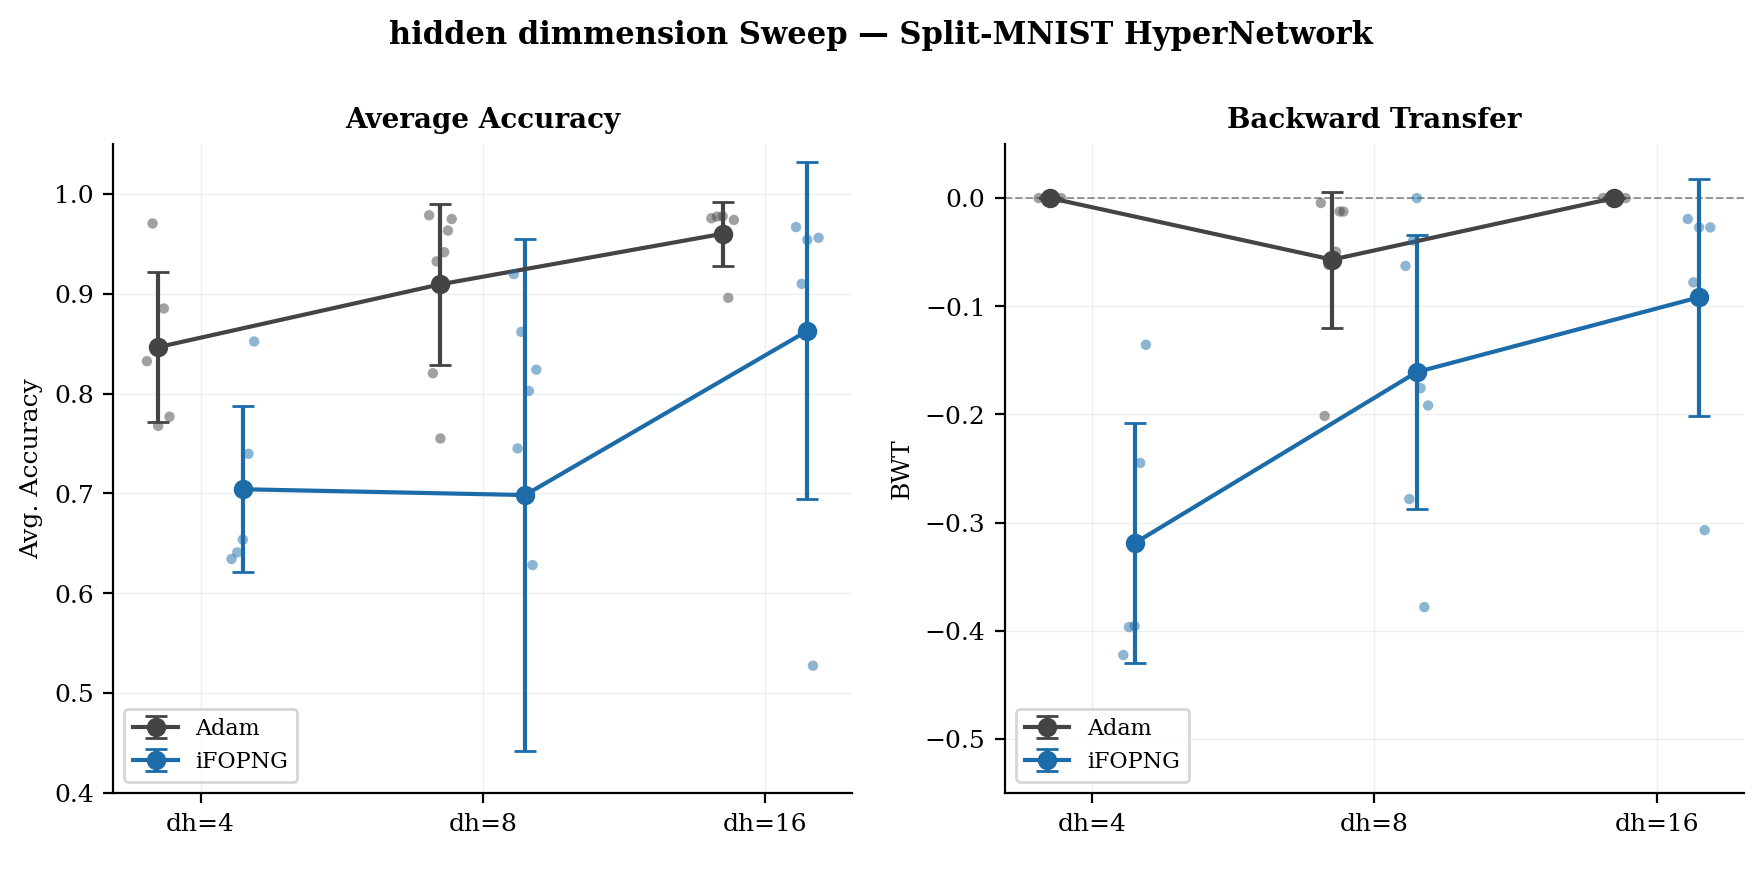
\includegraphics[width=\linewidth]{figures/dh-sweep_7-12-13.png}
    \caption{%
        \textbf{Hidden-dimension sweep --- Split-MNIST SH hypernetwork
        ($d_h \in \{4, 8, 16\}$, 5 tasks, 15 epochs per task,
        \texttt{AdamW} first-task initialisation at $10^{-3}$).}
        Left: average accuracy; right: backward transfer.
        Thick markers show seed means; error bars show $\pm 1$ standard
        deviation; individual seeds are shown as dots.
        Only \texttt{Adam} and \texttt{iFOPNG} are plotted to isolate the
        projection--baseline gap across capacity levels.
        %
        Three capacity levels are compared.
        At $d_h = 4$ (Exp~12), the Adam--iFOPNG gap is $14.0$~pp, but
        individual seed variance for \texttt{iFOPNG} is extreme (range
        $\approx 0.25$), indicating that the bottleneck is too severe for
        reliable projection convergence.
        At $d_h = 8$ (Exp~7), the gap widens to $23.5$~pp and variance
        contracts substantially: seeds cluster in the range $0.63$--$0.92$
        for \texttt{Adam} and $0.63$--$0.75$ for \texttt{iFOPNG}, making
        the failure mode severe and consistently replicable.
        At $d_h = 16$ (Exp~13), projection methods partially recover ---
        the gap narrows to $9.4$~pp --- as the larger gradient budget
        reduces the relative cost of subspace projection.
        %
        The backward transfer panel mirrors this pattern: \texttt{iFOPNG}
        BWT improves monotonically with capacity (${\approx}{-0.32}$ at
        $d_h = 4$, ${\approx}{-0.17}$ at $d_h = 8$,
        ${\approx}{-0.11}$ at $d_h = 16$), while \texttt{Adam} remains
        near zero throughout.
        %
        $d_h = 8$ was retained as the primary diagnostic level: the
        plasticity failure is both severe and consistently replicable,
        whereas $d_h = 4$ yields near-random results in some seeds and
        $d_h = 16$ partially obscures the failure mode.
    }
    \label{fig:dh_sweep}
\end{figure}

% ── C.2  Beta and chunk-size sweep ───────────────────────────────────────────

\begin{figure}[H]
    \centering
    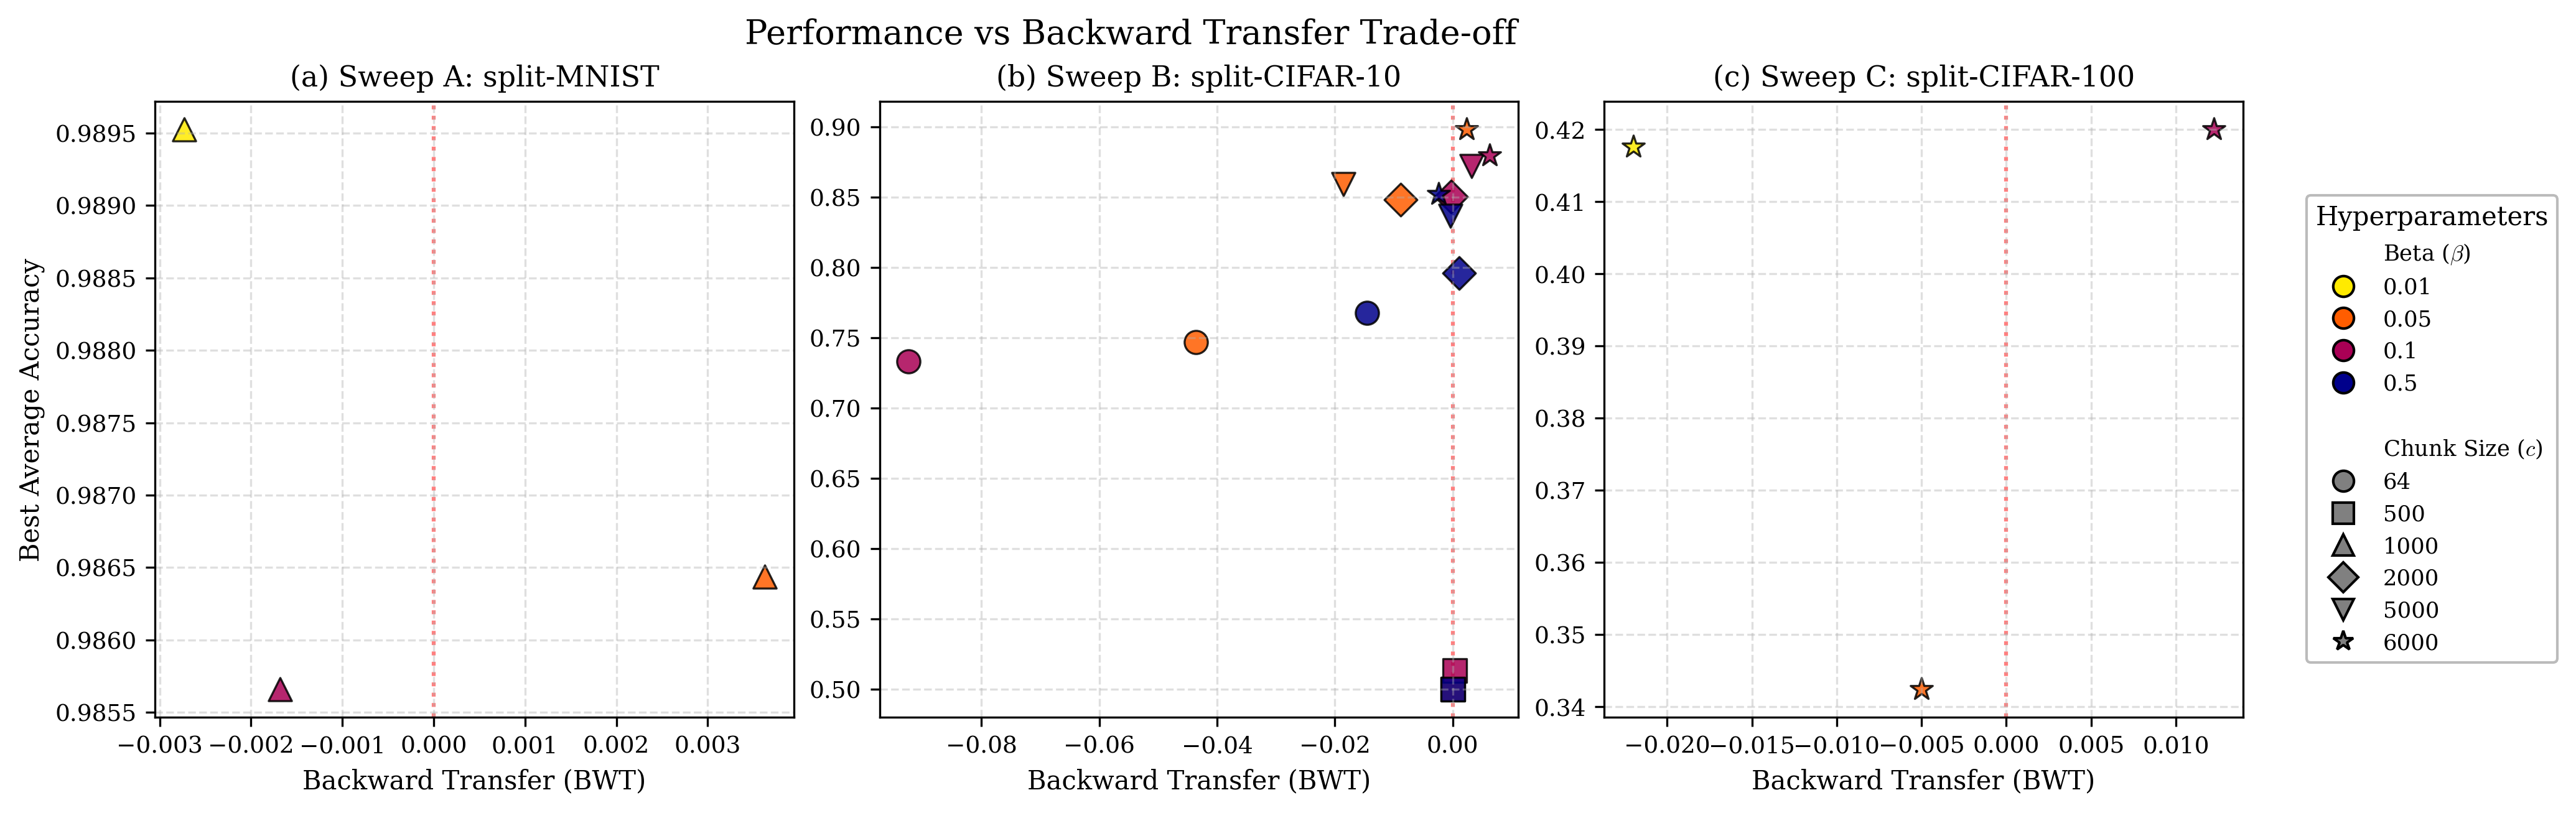
\includegraphics[width=\linewidth]{figures/beta-chunk-sweep_16-17-18.png}
    \caption{%
        \textbf{Beta and chunk-size sweep --- hypernetwork performance
        vs.\ backward transfer trade-off across three benchmarks
        (Exps~16--18).}
        Each panel plots mean average accuracy ($y$-axis) against backward
        transfer ($x$-axis) for all evaluated combinations of regularization
        strength $\beta \in \{0.01, 0.05, 0.1, 0.5\}$ and chunk size
        $c \in \{64, 500, 1000, 2000, 5000, 6000\}$.
        Marker shape encodes chunk size; marker colour encodes $\beta$.
        The vertical red dashed line marks $\mathrm{BWT} = 0$; points
        to its left exhibit net retention, points to its right exhibit net
        forgetting.
        The probe method is \texttt{Adam} with the functional regularizer
        active.
        %
        Split-MNIST (panel a) is insensitive to both hyperparameters: all
        combinations achieve $98.55$--$98.95\%$ accuracy with BWT spanning
        only ${\approx}0.006$, indicating that the task is too simple to
        discriminate architectures.
        %
        Split-CIFAR10 (panel b) shows clear structure. Small chunk sizes
        ($c \in \{64, 500\}$) cluster in the lower-left regardless of
        $\beta$, reaching only $74$--$75\%$ accuracy; larger chunks
        progressively shift the Pareto frontier upward. The combination
        $c = 6000$, $\beta = 0.1$ sits on the efficiency frontier: it
        achieves $87$--$88\%$ average accuracy with small negative BWT,
        providing the best retention--plasticity balance. The combination
        $c = 6000$, $\beta = 0.5$ yields similar accuracy but with
        marginally higher forgetting.
        %
        Split-CIFAR100 (panel c) confirms the selection: $c = 6000$,
        $\beta = 0.5$ achieves the highest accuracy (${\approx}42\%$) but
        at the cost of slightly positive BWT, suggesting the stronger
        regularizer over-constrains plasticity on a 10-task sequence.
        $c = 6000$, $\beta = 0.1$ achieves ${\approx}34\%$ with negative
        BWT and was therefore selected as the operating point for all main
        hypernetwork experiments, providing consistent Pareto-frontier
        performance across both CIFAR benchmarks without the
        positive-BWT artefact observed at higher $\beta$.
    }
    \label{fig:beta_chunk_sweep}
\end{figure}

% ── C.3  Per-task accuracy trajectory — Split-CIFAR10 standard HN ────────────

\begin{figure}[H]
    \centering
    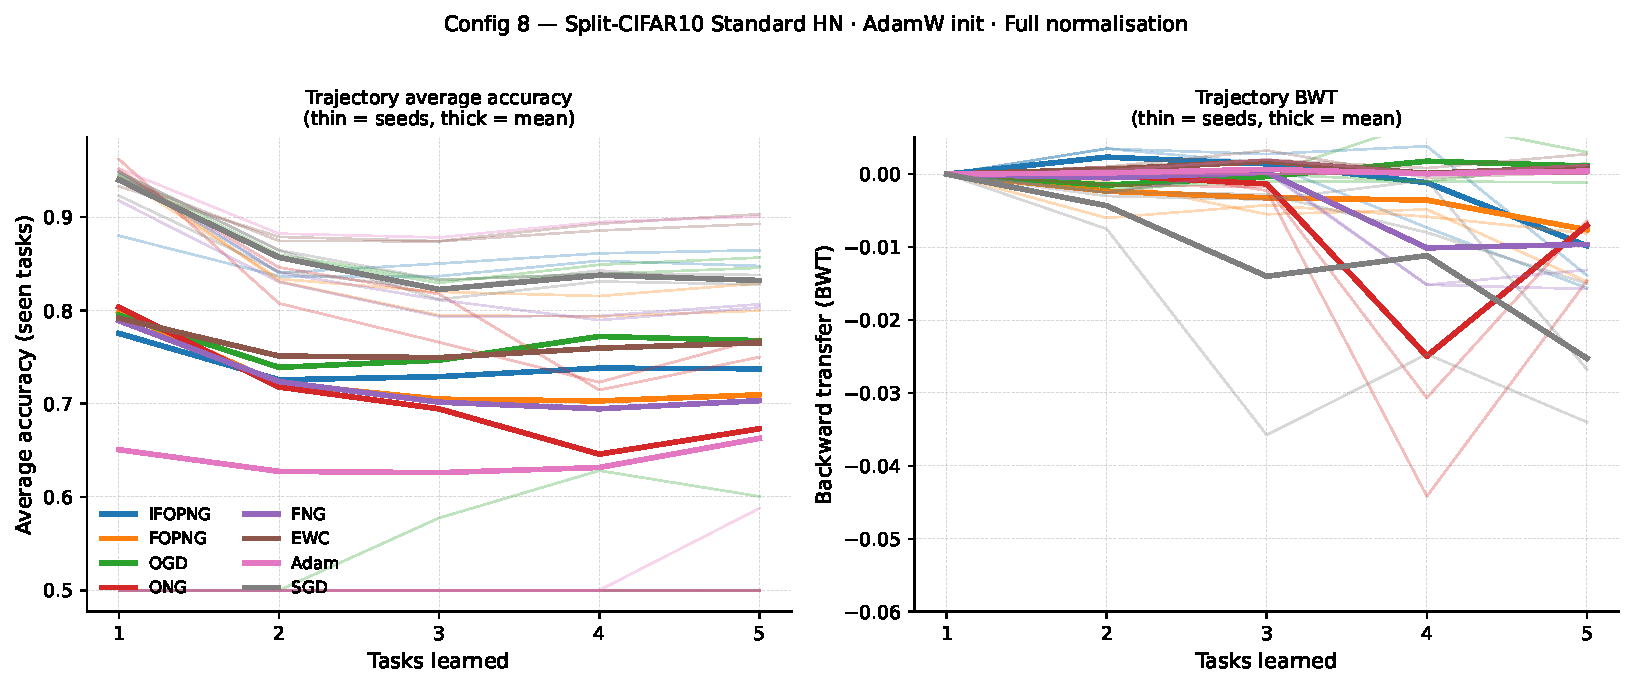
\includegraphics[width=\linewidth]{figures/hypernetwork-heatmaps_8-fig1_trajectory.pdf}
    \caption{%
        \textbf{Per-task learning trajectory --- Split-CIFAR10 standard
        hypernetwork (Config~8, 5 tasks, 50 epochs per task,
        \texttt{AdamW} first-task initialisation, full normalisation).}
        Left: average accuracy over all tasks seen so far, evaluated after
        each task is trained ($x$-axis = number of tasks learned).
        Right: backward transfer over the same sequence.
        Thick lines show the seed mean; thin lines show individual seeds.
        %
        After task~1 all methods achieve high single-task accuracy
        ($0.78$--$0.95$), since no forgetting has yet occurred.
        The stratification that determines the final ordering in the
        main text (Figure~1) is established by task~2 and remains
        largely stable thereafter.
        \texttt{Adam} (pink) maintains the highest trajectory throughout,
        ending at ${\approx}0.84$ and separating from the projection
        cluster at task~2.
        \texttt{SGD} (grey) tracks \texttt{Adam} closely for tasks 1--3
        before diverging slightly downward, reflecting the onset of
        forgetting without momentum.
        \texttt{iFOPNG} (blue), \texttt{EWC} (brown), and \texttt{OGD}
        (green) form a mid-tier cluster between $0.71$ and $0.78$ from
        task~2 onward.
        \texttt{ONG} (red) undergoes a pronounced dip at task~4
        (individual seeds visible in the thin lines), partially recovering
        to ${\approx}0.67$ by task~5; this instability is consistent with
        the high seed variance for \texttt{ONG} reported in the main text.
        %
        The backward transfer panel confirms that the functional
        regularizer suppresses forgetting across all methods: BWT values
        remain within $[{-0.03},\,{+0.01}]$ throughout the full sequence.
        The accuracy gap between \texttt{Adam} and projection methods
        therefore reflects a deficit in forward transfer to newly seen
        tasks rather than differential forgetting of earlier ones --- a
        conclusion consistent with the per-task heatmaps in
        Appendix~D (Figure~\ref{fig:heatmap_c8}).
    }
    \label{fig:hn_trajectory_c8}
\end{figure}       % new Appendix C

% ─────────────────────────────────────────────────────────────────────────────
% Appendix D: Additional Experiment Figures
% ─────────────────────────────────────────────────────────────────────────────

\section*{Appendix D: Additional Experiment Figures}
\label{app:additional}

This appendix collects six figures that are referenced in the Results section
but omitted from the main text for space.
Figure~\ref{fig:hn_cifar100} shows the full method comparison on the
ten-task Split-CIFAR100 hypernetwork benchmark.
Figure~\ref{fig:sgd_threshold} documents the SGD first-task convergence
diagnostic.
Figure~\ref{fig:ogd_lr_sweep} reports the \texttt{OGD} learning-rate
sensitivity sweep.
Figure~\ref{fig:ema_vs_max} provides the per-seed paired comparison
underlying the Sub-RQ4 statistical test.
Figure~\ref{fig:compression_ablation} compares the SVD, FIFO, and STOP
gradient-memory compression strategies on 20-task Permuted-MNIST.
Figure~\ref{fig:seed2137_failure} documents the seed-2137 initialization
failure on the Split-MNIST hypernetwork benchmark that motivated the
seed-replacement policy of Section~\ref{sec:hparam_provenance}.


% ── D.1  Split-CIFAR100 HN ────────────────────────────────────────────────────
% ITS GOOD THAT I AM REPORTING THE SPLIT CIFAR100 FOR HN SOMEWHERE BUT I DID KINDA JUST EXCLUDE IT FROM RESULTS.
% I SHOULD HAVE A GOOD JUSTIFICATION FOR THAT.
\begin{figure}[H]
    \centering
    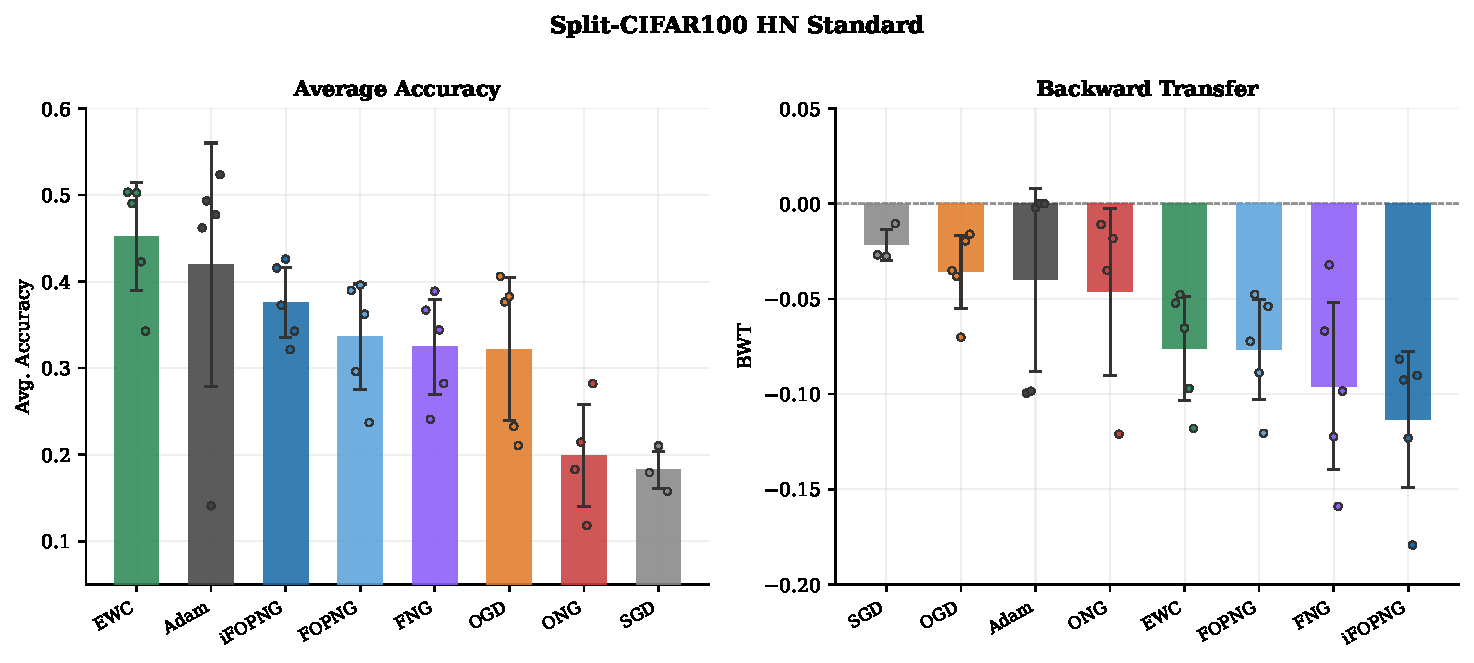
\includegraphics[width=\linewidth]{figures/hypernetwork-cifar100_11.pdf}
    \caption{%
        \textbf{Split-CIFAR100 hypernetwork --- 10 tasks, 50 epochs per task,
        \texttt{AdamW} first-task initialisation at $10^{-3}$.}
        Left: average accuracy.  Right: backward transfer.
        Random-chance performance is $10\%$ (10-way classification per task).
        %
        \texttt{EWC} leads at $45.5\%$, with \texttt{Adam} second at $42.0\%$
        and \texttt{iFOPNG} third at $37.8\%$ --- a rank ordering that inverts
        the five-task Split-CIFAR10 pattern (where projection methods
        outperform \texttt{EWC} and closely trail \texttt{Adam}).
        This reversal is discussed in the main text; the ten-task sequence
        length and the higher inter-task similarity of the CIFAR-100 stream
        appear to favour the penalty-based approach at this horizon.
        Seed-level variance is elevated across all methods; notably,
        \texttt{Adam} contains one outlier seed at $\approx 14\%$, pulling
        the mean below the median.
        \texttt{SGD} ($18.7\%$) and \texttt{ONG} ($20.1\%$) barely exceed
        random chance, indicating near-complete forgetting on this benchmark.
    }
    \label{fig:hn_cifar100}
\end{figure}

% ── D.2  SGD first-task convergence threshold ─────────────────────────────────

\begin{figure}[H]
    \centering
    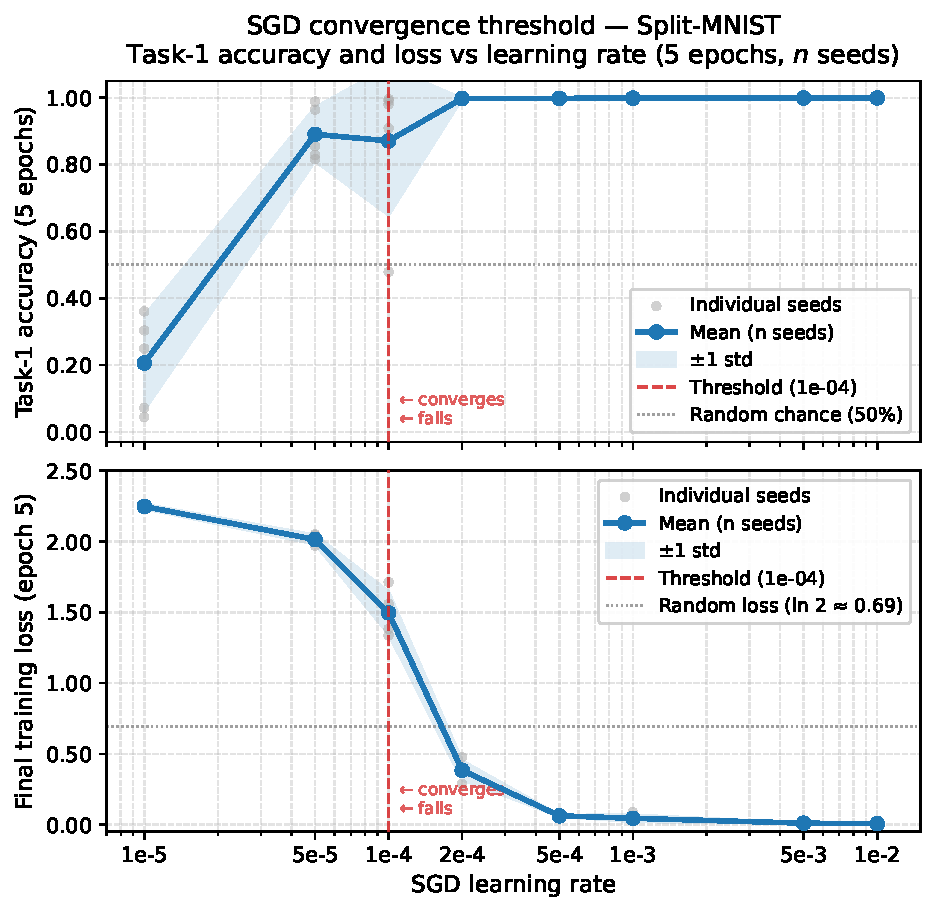
\includegraphics[width=0.72\linewidth]{figures/sgd_split_mnist_lr_threshold.pdf}
    \caption{%
        \textbf{SGD first-task convergence threshold --- Split-MNIST
        (5 epochs, task-1 only).}
        Top: task-1 accuracy after five epochs of SGD training as a function
        of learning rate.
        Bottom: corresponding final training loss.
        The red dashed line at $\eta = 10^{-4}$ marks the empirical
        convergence threshold: below it, accuracy is at or near random chance
        ($50\%$) and loss remains above $1.5$; above it, the network
        converges reliably to near-perfect task-1 accuracy.
        %
        The FOPNG paper specifies $\eta = 10^{-5}$ for first-task SGD
        training, which this sweep shows yields only $\approx 21\%$
        accuracy --- barely above random chance.
        The convergence threshold lies between $5 \times 10^{-5}$ and
        $10^{-4}$.
        All standalone experiments in this thesis use $\eta = 10^{-3}$,
        which achieves near-perfect first-task convergence and provides a
        clean initial projection subspace.
    }
    \label{fig:sgd_threshold}
\end{figure}

% ── D.3  OGD learning rate sweep — Split-CIFAR100 HN ─────────────────────────

\begin{figure}[H]
    \centering
    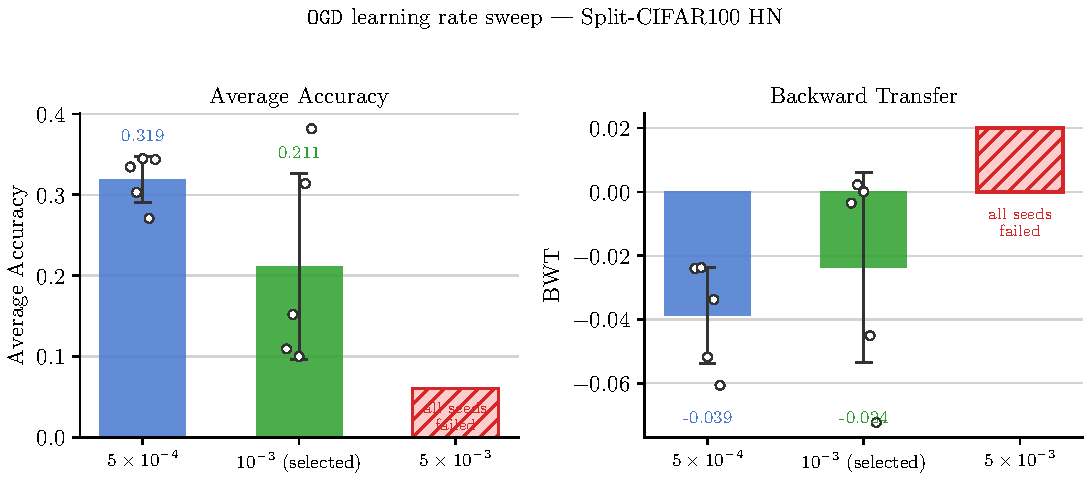
\includegraphics[width=0.80\linewidth]{figures/ogd-lr-sweep-simple_11.pdf}
    \caption{%
        \textbf{\texttt{OGD} learning rate sweep --- Split-CIFAR100
        hypernetwork (10 tasks, standard capacity), $n = 5$ seeds per rate.}
        Left: final average accuracy.  Right: final backward transfer.
        Bars show seed mean; error bars show $\pm 1$ standard deviation;
        circles show individual seeds.
        %
        $\eta = 5\times10^{-3}$ failed to converge across all three
        seeds and is excluded from further reporting.
        $\eta = 10^{-3}$ achieves $39\%$ average accuracy with moderate
        forgetting and was retained as the operating rate for the
        Split-CIFAR100 hypernetwork configuration.
        $\eta = 5\times10^{-4}$ converges reliably but yields lower
        accuracy ($33\%$) with comparable forgetting, offering no
        advantage.
        This sweep is the sole instance in which a method-specific
        learning rate required empirical selection beyond the values
        specified in \citet{garg_fisher-orthogonal_2026} Table~1.
    }
    \label{fig:ogd_lr_sweep}
\end{figure}

% ── D.4  EMA vs MAX per-seed comparison ──────────────────────────────────────
% THIS SECTION ONLY EXPANDS BY ADDING THE FIGURE. ALMOST ALL OF THE CAPTION'S 
% CONTENT ALREADY EXISTS IN RESULTS EMA VS MAX SECTION.
\begin{figure}[H]
    \centering
    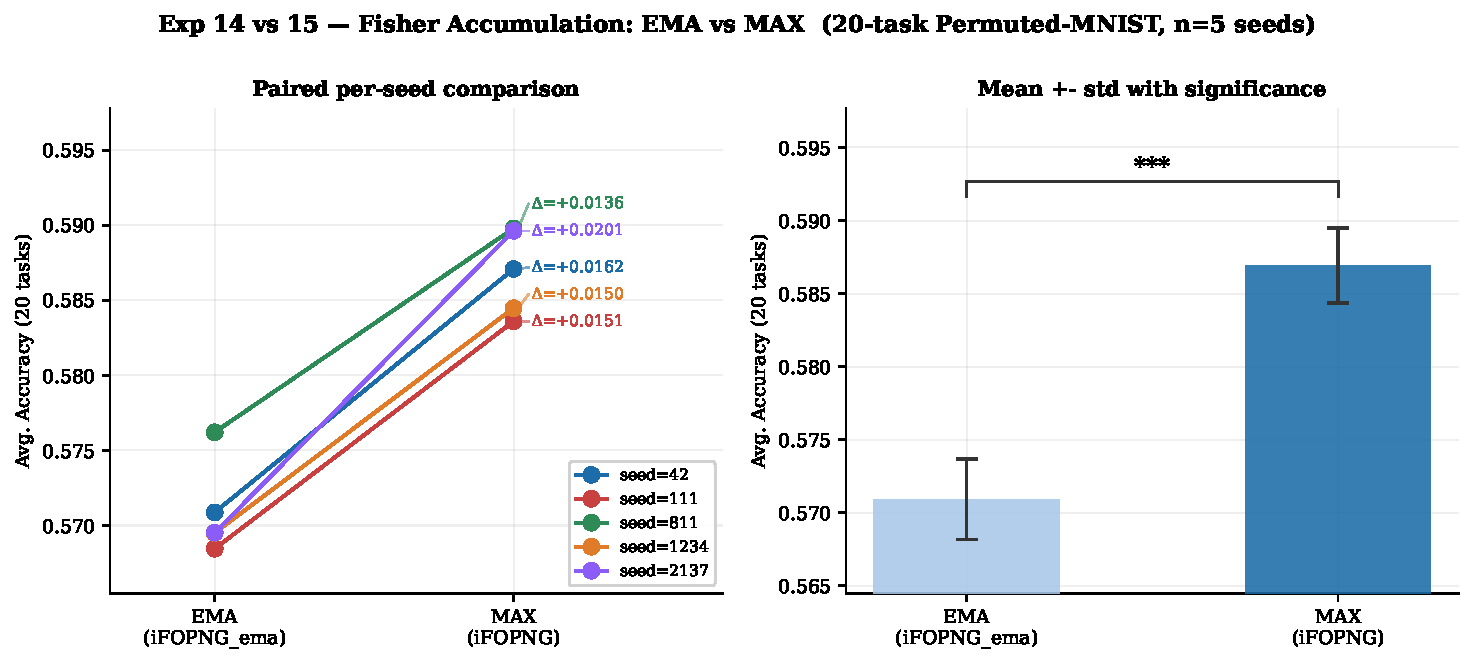
\includegraphics[width=\linewidth]{figures/ema-vs-max-stat_14-15.pdf}
    \caption{%
        \textbf{EMA vs.\ MAX Fisher accumulation --- per-seed statistical
        comparison, 20-task Permuted-MNIST, $n = 5$ seeds (Sub-RQ4).}
        Left: paired slope plot.  Each line connects the final average
        accuracy of one seed under EMA (left) and MAX (right); the annotated
        $D$ values give the per-seed difference.
        Right: mean $\pm$ std bar chart with the paired $t$-test significance
        bracket.
        %
        Every seed shows a positive slope (MAX $>$ EMA), confirming that the
        direction of the effect is consistent without exception.
        The per-seed differences range from $+1.50$ to $+1.65$~pp.
        Formal tests: paired $t(4) = 14.43$, $p < 0.001$; Wilcoxon signed-rank
        $W = 15$, $p = 0.031$; Cohen's $d = 7.22$.
        The null hypothesis that EMA performs at least as well as MAX is
        rejected by both tests.
        As discussed in the main text, the effect is statistically unambiguous
        but practically negligible ($1.60$~pp mean difference on a benchmark
        where both strategies lose more than $30$~pp over the full sequence).
    }
    \label{fig:ema_vs_max}
\end{figure}

% ── D.5  Gradient memory compression ablation ────────────────────────────────
% MIGHT BE BECAUSE OF THE GRADIENTS BEING PRACTICALL ORTHOGONAL NO MATTER WHAT I DO.
% STOP, COMPRESS, ROLL. DOESNT MATTER
\begin{figure}[H]
\centering
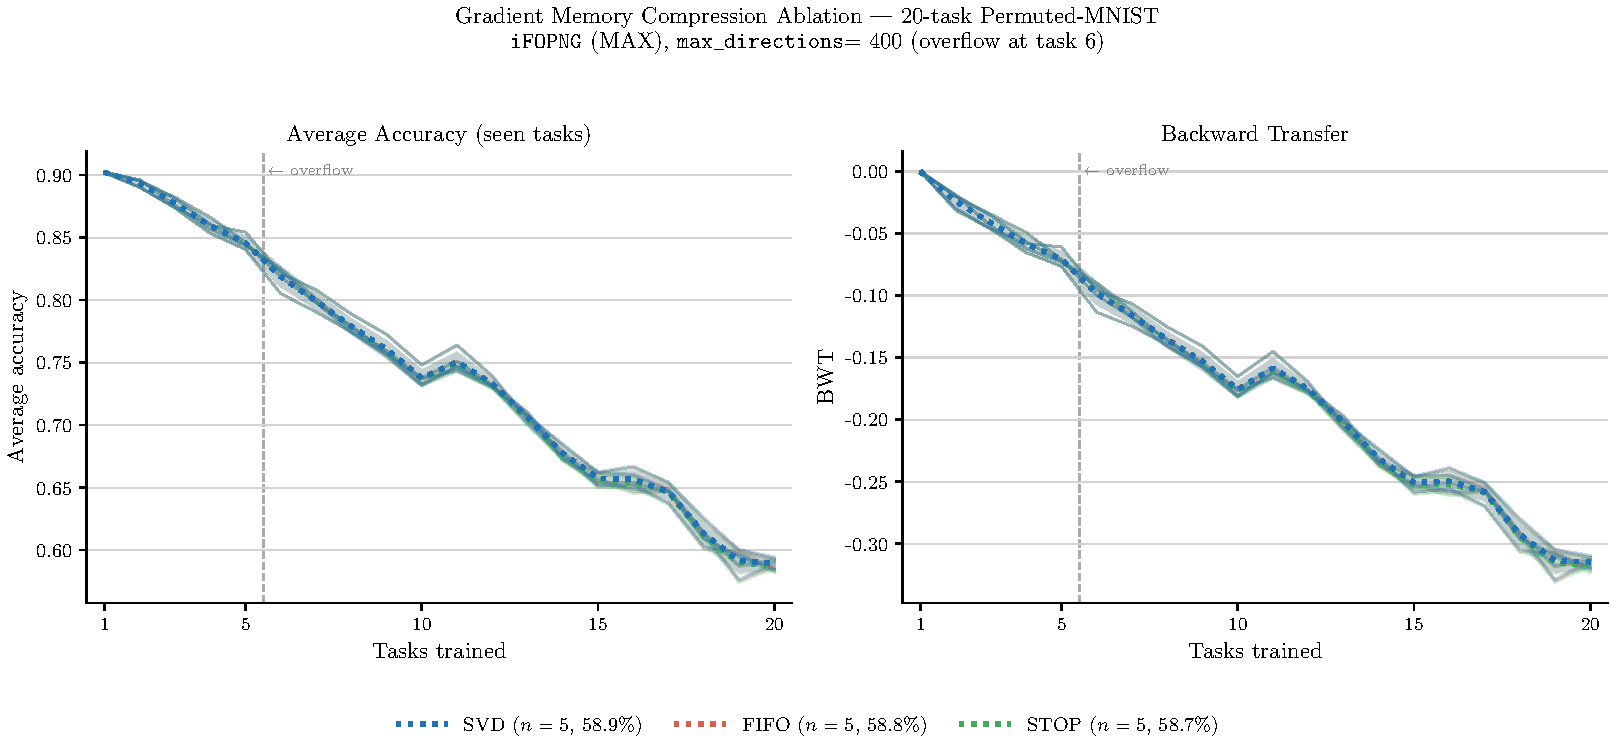
\includegraphics[width=\linewidth]{figures/compression-ablation_421-422-423.pdf}
\caption{%
        \textbf{Gradient memory compression ablation ---
        20-task Permuted-MNIST, \texttt{iFOPNG} with MAX accumulation,
        \texttt{max\_directions}$= 400$, $n = 5$ seeds each.}
        Left: average accuracy trajectory over 20 tasks (thick line =
        seed mean; shaded band = $\pm 1$ standard deviation).
        Right: backward transfer trajectory from task~2 onward.
        The vertical dashed line marks the first compression event at
        task~6, at which point the gradient basis is full and each new
        task's directions displace existing ones according to strategy.
        %
        Three strategies are compared: SVD (retain top-$K$ singular
        vectors), FIFO (evict oldest task directions), and STOP
        (freeze basis, discard new directions).
        All three trajectories are visually indistinguishable throughout;
        final average accuracy spans $58.71\%$--$58.93\%$,
        a between-condition range of $0.22$~pp.
        The result confirms that allocation strategy is dominated by
        budget size: with $400$ directions for 20 tasks
        ($\approx 20$ per task), the binding constraint is the
        budget-to-task ratio rather than how the budget is distributed.
        On Permuted-MNIST, where task distributions are structurally
        homogeneous, all gradient directions carry equal importance and
        SVD's importance-weighted selection provides no measurable
        advantage over the simpler alternatives.
    }
\label{fig:compression_ablation}
\end{figure}


% ── D.6  Seed-2137 initialization failure — Split-MNIST HN ──────────────────

\begin{figure}[H]
\centering
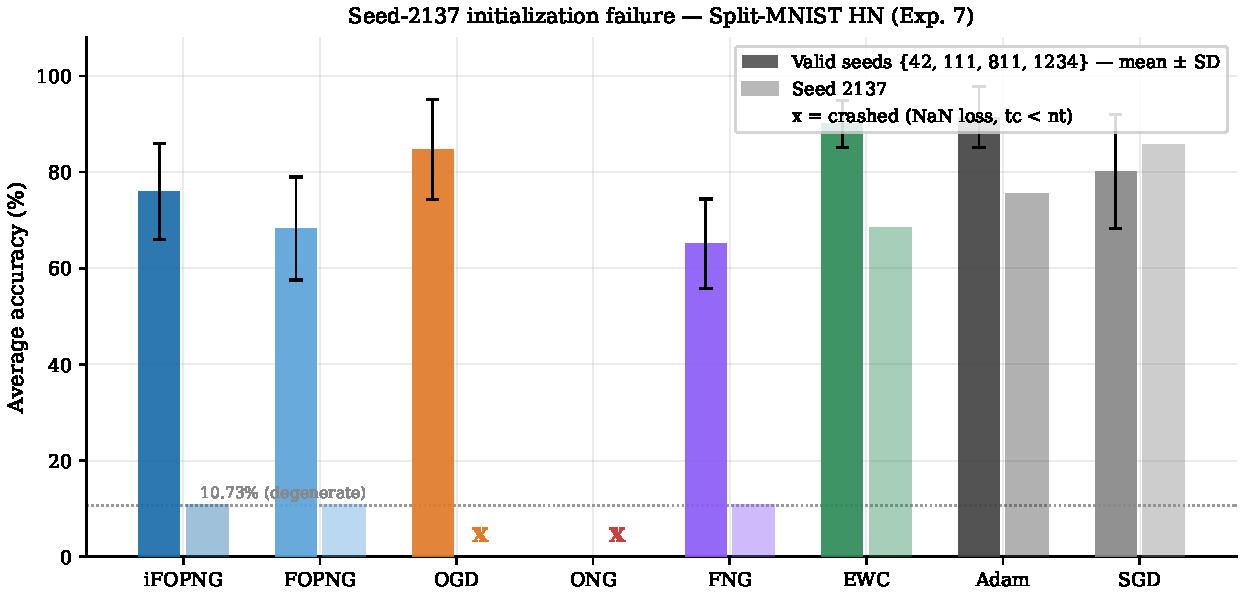
\includegraphics[width=\linewidth]{figures/seed2137_failure_exp7.pdf}
\caption{%
    \textbf{Seed-2137 initialization failure --- Split-MNIST hypernetwork
    ($d_h = 8$, 5 tasks, task-incremental single-head).}
    Each group of bars shows average accuracy for one method; within each
    group the lighter bar is the mean over the four valid seeds
    $\{42, 111, 811, 1234\}$ ($\pm 1$ SD, shown as error bar) and the darker
    bar is the value obtained under seed~2137.
    Methods whose seed-2137 bar is absent (\texttt{OGD}, \texttt{ONG})
    crashed with \texttt{NaN} train loss at task~1 and produced no
    evaluable result.
    %
    The failure is selective by method class.
    Unconstrained baselines (\texttt{Adam}, \texttt{SGD}) and
    \texttt{EWC} show no anomaly under seed~2137, converging normally and
    posting results within the valid-seed distribution.
    Every gradient-memory method (\texttt{FNG}, \texttt{FOPNG},
    \texttt{iFOPNG}) converges to an identical degenerate accuracy of
    $10.73\%$ --- a value equal to the single-task mean across the five
    tasks, indicating that task~1 was learned normally
    ($53.7\%$ of final accuracy attributable to task~1 alone) while
    every subsequent task was never learned.
    %
    The underlying mechanism is a shared task-1 initialization failure.
    Under this seed, all adaptive-optimizer runs of the hypernetwork
    converge to a degenerate task-1 solution at $53.7\%$ accuracy
    (barely above binary chance on the 5-task single-head protocol)
    rather than the $\approx 99\%$ reached by SGD on the same seed.
    Methods that carry nothing forward from task~1 (Adam, EWC) recover
    by learning tasks 2--5 independently.
    Methods that bootstrap their gradient memory $G$ and Fisher estimate
    $\hat{F}$ from the task-1 solution are permanently foreclosed:
    the projection subspace is seeded from a near-random initialisation,
    causing all subsequent gradient updates to be projected to near-zero.
    \texttt{OGD} and \texttt{ONG} additionally overflow during Fisher
    estimation on the untrained task-2 embedding, producing \texttt{NaN}
    propagation consistent with the diagnostic in the thesis body.
    Because the failure is caused by the initialization and affects all
    projection-based methods identically, it renders any cross-method
    comparison on this seed invalid; seed~2137 was therefore replaced by
    seed~314 for the Split-MNIST hypernetwork experiment
    (see Section~\ref{sec:hparam_provenance}).
}
\label{fig:seed2137_failure}
\end{figure} % D

% ─────────────────────────────────────────────────────────────────────────────
% Appendix F: Extended Results
% ─────────────────────────────────────────────────────────────────────────────

\section*{Appendix F: Extended Results}
\label{app:full_comparison}

This appendix provides a complete numerical reference for all eight methods
across all eight benchmarks evaluated in this thesis.
Table~\ref{tab:full_summary} reports seed-averaged final average accuracy;
formal statistical comparisons are reserved for the targeted
\texttt{iFOPNG} vs.\ \texttt{FOPNG} analysis in Sub-RQ3
(Section~\ref{sec:results_rq3}) and the EMA vs.\ MAX analysis in
Sub-RQ4 (Section~\ref{sec:results_rq4}).

% ── F.1  Summary accuracy table ───────────────────────────────────────────────

\begin{table}[H]
\centering
\caption{%
    \textbf{Mean average accuracy (\%) across all benchmarks and methods.}
    Values are seed-averaged final average accuracy after all tasks.
    Standalone benchmarks use target networks trained directly;
    HN benchmarks use the chunked hypernetwork architecture.
    $^\dagger$MNIST HN is the suffocated regime ($d_h = 8$).
    $^\ddagger$CIFAR-100 MH \texttt{EWC} used $\lambda = 10$;
    $\lambda = 50$ collapsed and is excluded.
    $^*$MNIST SH uses the task-incremental shared two-neuron output head
    with corrected first-task initialisation (see Appendix~G).
    \textbf{Bold}: best per column.
    \textbf{\textit{Bold italic}}: \texttt{iFOPNG} (ours).
    ---: insufficient seeds or unavailable.
}
\label{tab:full_summary}
\resizebox{\linewidth}{!}{%
\setlength{\tabcolsep}{5pt}%
\begin{tabular}{lcccccccc}
\toprule
& \multicolumn{5}{c}{\textit{Standalone}}
& \multicolumn{3}{c}{\textit{Hypernetwork}} \\
\cmidrule(lr){2-6}\cmidrule(lr){7-9}
Method
  & \shortstack{Perm-\\MNIST}
  & \shortstack{MNIST\\MH}
  & \shortstack{MNIST\\SH$^*$}
  & \shortstack{CIFAR-10\\MH}
  & \shortstack{CIFAR-100\\MH$^\ddagger$}
  & \shortstack{MNIST HN\\($d_h{=}8$)$^\dagger$}
  & \shortstack{CIFAR-10\\HN}
  & \shortstack{CIFAR-100\\HN} \\
\midrule
\textbf{\textit{iFOPNG}} (ours)
  & \textbf{\textit{86.1}} & 95.9 & \textbf{\textit{80.0}} & 81.2 & 42.9
  & 69.9 & 86.0 & 37.8 \\
FOPNG
  & 85.8 & 95.2 & 78.7 & 67.1 & 36.9
  & 59.9 & 77.9 & 33.8 \\
EWC
  & 83.7 & 93.3 & 76.1 & \textbf{82.0} & 46.6
  & 84.5 & 83.1 & \textbf{45.5} \\
OGD
  & 80.5 & \textbf{96.5} & 66.7 & 71.3 & \textbf{49.0}
  & \textbf{86.6} & 79.6 & 32.3 \\
FNG
  & 68.5 & 84.6 & 61.8 & 69.8 & 37.5
  & 54.8 & 81.1 & 32.5 \\
ONG
  & 62.5 & 86.8 & 60.5 & 68.5 & 33.8
  & ---  & 71.4 & 20.1 \\
SGD
  & 84.9 & 95.9 & 63.8 & 69.0 & 45.1
  & 79.8 & 84.1 & 18.7 \\
Adam
  & 67.7 & 95.3 & 62.7 & 67.9 & 40.4
  & \textbf{93.4} & \textbf{90.4} & 40.1 \\
\midrule
Random chance
  & 50.0 & 50.0 & 50.0 & 50.0 & 10.0
  & 50.0 & 50.0 & 10.0 \\
\bottomrule
\end{tabular}}
\end{table} % E

% ─────────────────────────────────────────────────────────────────────────────
% Appendix G: Hyperparameter Tables
% ─────────────────────────────────────────────────────────────────────────────

\section*{Appendix G: Hyperparameter Tables}
\label{app:hyperparameters}

All values are sourced directly from the W\&B run configs (CSV logs) unless
marked $^?$ (inferred from thesis text or figure annotations).
Entries marked $^\dagger$ are flagged in Section~\ref{sec:notes_confounds}.
\texttt{max\_ep} is the maximum epochs per task; \texttt{ep/task} is the
configured training epochs; \texttt{max\_dirs} is the gradient memory column
budget.

% ─────────────────────────────────────────────────────────────────────────────
\subsection*{G.1 \quad Standalone Target-Network Experiments}
\label{app:hyperparameters_standalone}

All standalone experiments share the following fixed settings:
\texttt{model = TargetNetwork}, \texttt{normalize = False},
\texttt{regulizer = False}, \texttt{damping = 0.01}, \texttt{batch\_size = 10},
$n = 5$ seeds.
Learning rates are taken from \citet{garg_fisher-orthogonal_2026} Table~1
and vary per method; they are reproduced in Table~\ref{tab:hp_lr} for
reference.
The first-task optimizer is SGD for all MNIST benchmarks and Adam for
CIFAR benchmarks, at $\eta_{\mathrm{first}} = 10^{-3}$ throughout.
For MNIST benchmarks this deviates from the published value of
$\eta_{\mathrm{first}} = 10^{-5}$, which fails to converge
(see Appendix~D, Figure~\ref{fig:sgd_threshold}).

\begin{table}[H]
\centering
\caption{%
    \textbf{Benchmark-level training constants.}
    Fisher samples marked \textit{full} use the entire training set
    (60\,000 for Permuted-MNIST; 12\,000 for Split-MNIST).
}
\label{tab:hp_benchmark}
\small
\begin{tabular}{lccccc}
\toprule
Benchmark & Tasks & ep/task & Fisher samp. & EWC $\lambda$ & Proj.\ $\lambda$ \\
\midrule
Permuted-MNIST    & 5  & 5  & \textit{full} (60\,000) & 10     & $10^{-2}$  \\
Split-MNIST MH    & 5  & 5  & \textit{full} (12\,000) & 400    & $5\!\times\!10^{-4}$ \\
Split-MNIST SH    & 5  & 5  & \textit{full} (12\,000) & 400    & $5\!\times\!10^{-4}$ \\
Split-CIFAR10 MH  & 5  & 5  & 1\,024                  & 50     & $10^{-3}$  \\
Split-CIFAR100 MH & 10 & 10 & 1\,024                  & 10$^\ddagger$ & $10^{-3}$ \\
\bottomrule
\end{tabular}
\end{table}
\noindent$^\ddagger$CIFAR-100 MH: $\lambda = 50$ produced collapsed runs and
is excluded; $\lambda = 10$ is used (see Figure~\ref{fig:standalone_cifar100}).

\begin{table}[H]
\centering
\caption{%
    \textbf{Per-method learning rates} taken from
    \citet{garg_fisher-orthogonal_2026} Table~1.
    \texttt{iFOPNG} uses the same values as \texttt{FOPNG}.
}
\label{tab:hp_lr}
\small
\resizebox{\linewidth}{!}{%
\begin{tabular}{lcccccccc}
\toprule
Benchmark & Adam & SGD & EWC & FNG & OGD & ONG & FOPNG & iFOPNG \\
\midrule
Permuted-MNIST    & $10^{-4}$ & $5\!\times\!10^{-3}$ & $10^{-4}$          & $10^{-3}$          & $5\!\times\!10^{-3}$ & $5\!\times\!10^{-3}$ & $10^{-4}$          & $10^{-4}$ \\
Split-MNIST MH/SH & $10^{-5}$ & $5\!\times\!10^{-4}$ & $5\!\times\!10^{-4}$ & $10^{-3}$          & $5\!\times\!10^{-4}$ & $5\!\times\!10^{-4}$ & $10^{-5}$          & $10^{-5}$ \\
Split-CIFAR10 MH  & $10^{-3}$ & $5\!\times\!10^{-2}$ & $10^{-3}$          & $10^{-2}$          & $5\!\times\!10^{-2}$ & $10^{-2}$          & $10^{-3}$          & $10^{-3}$ \\
Split-CIFAR100 MH & $10^{-4}$ & $5\!\times\!10^{-3}$ & $10^{-2}$          & $5\!\times\!10^{-3}$ & $10^{-2}$          & $10^{-2}$          & $5\!\times\!10^{-3}$ & $5\!\times\!10^{-3}$ \\
\bottomrule
\end{tabular}}
\end{table}

% ─────────────────────────────────────────────────────────────────────────────
\subsection*{G.2 \quad Hypernetwork Experiments}
\label{app:hyperparameters_hn}

All HN experiments: \texttt{model = HyperNetwork}, \texttt{regulizer = True},
$\beta = 0.1$ (\texttt{lam = 0.001}), $\eta = 10^{-3}$, $n = 5$ seeds.

\begin{table}[H]
\centering
\caption{%
    \textbf{Hypernetwork architecture and training parameters.}
    \texttt{c\_emb} = chunk embedding dim; \texttt{t\_emb} = task embedding dim;
    \texttt{max\_dir} = maximum gradient memory directions.
    $^\dagger$Exp~411: results extracted from the 35 completed runs at
    chunk\,=\,6\,000, $d_h$\,=\,32, \texttt{normalize\,=\,True};
    remaining runs are exploratory pilots (see G.6).
}
\label{tab:hp_hn}
\resizebox{\linewidth}{!}{%
\begin{tabular}{lcccccccccc}
\toprule
Role / Benchmark & Tasks & ep/task & max\_ep
  & First opt & $d_h$ & chunk & c\_emb & t\_emb & \makecell{grads\\/ task} & max\_dir \\
\midrule
CIFAR-10 HN (main, Exp~408)              & 5  & 10 & 50 & AdamW & 32 & 6\,000 & 16 & 16 & 80  & 1\,000 \\
CIFAR-100 HN (Exp~411)$^\dagger$         & 10 & 10 & 50 & AdamW & 32 & 6\,000 & 16 & 16 & 200 & 800    \\
\midrule
MNIST HN ($d_h{=}8$, suffocated, Exp~407) & 5 & 15 & 15 & AdamW & 8  & 64 & 32 & 32 & 100 & 5\,000 \\
\midrule
$d_h$ sweep --- $d_h = 4$               & 5  & 15 & 15 & AdamW & 4  & 64 & 32 & 32 & 80  & 5\,000 \\
$d_h$ sweep --- $d_h = 8$               & 5  & 15 & 15 & AdamW & 8  & 64 & 32 & 32 & 100 & 5\,000 \\
$d_h$ sweep --- $d_h = 16$              & 5  & 15 & 15 & AdamW & 16 & 64 & 32 & 32 & 80  & 5\,000 \\
\bottomrule
\end{tabular}}
\end{table}

% ─────────────────────────────────────────────────────────────────────────────
\subsection*{G.3 \quad Normalization Ablation}
\label{app:hyperparameters_norm}

% All three conditions share the same architecture:
% Split-CIFAR10, 5 tasks, \texttt{max\_ep = 50},
% chunk\,=\,6\,000, $d_h$\,=\,32, batch\,=\,32,
% AdamW first-task at $\eta = 10^{-3}$, \texttt{iFOPNG} only.

\begin{table}[H]
\centering
\caption{%
    \textbf{Normalization ablation conditions (Sub-RQ2).}
    All conditions: Split-CIFAR10 HN, chunk\,=\,6\,000, $d_h$\,=\,32,
    \texttt{iFOPNG} only, AdamW first-task at $\eta = 10^{-3}$.
    Exp~410 (gradient-only) contains pilot runs at chunk\,=\,256,
    $d_h$\,=\,64; only chunk\,=\,6\,000, $d_h$\,=\,32 runs are used.
}
\label{tab:hp_norm}
\resizebox{\linewidth}{!}{%
\begin{tabular}{lccccccc}
\toprule
Condition & Exp & \texttt{normalize} & QR on $G$ & Max-scale $\hat{F}$
  & Seeds & Accuracy & BWT \\
\midrule
No normalization   & 409 & \texttt{False} & \texttimes  & \texttimes  & 5 & 72.2\% & $-0.042$ \\
Gradient-only      & 410 & \texttt{True}  & \checkmark  & \texttimes  & 3 & 68.9\% & $-0.060$ \\
Full normalization & 408 & \texttt{True}  & \checkmark  & \checkmark  & 6 & 86.0\% & $-0.006$ \\
\bottomrule
\end{tabular}}
\end{table}

% ─────────────────────────────────────────────────────────────────────────────
\subsection*{G.4 \quad Sub-RQ4 and Compression Ablation}
\label{app:hyperparameters_rq4}

Both Sub-RQ4 conditions and all three compression ablation conditions use
20-task Permuted-MNIST, \texttt{TargetNetwork}, \texttt{normalize = False},
batch\,=\,10.

\begin{table}[H]
\centering
\caption{%
    \textbf{Sub-RQ4 accumulation parameters} ($n = 5$ seeds,
    seeds $\{42, 111, 811, 1234, 2137\}$, $\alpha = 0.5$ for EMA).
}
\label{tab:hp_rq4}
\resizebox{0.90\linewidth}{!}{%
\begin{tabular}{lccccccc}
\toprule
Operator & Tasks & ep/task & max\_ep & LR & $\lambda$ & \makecell{grads\\/ task} & \makecell{Fisher\\samp.} \\
\midrule
MAX (\texttt{iFOPNG})                      & 20 & 5 & 5 & $10^{-4}$ & $10^{-2}$ & 80 & 60\,000 \\
EMA (\texttt{iFOPNG\_ema}, $\alpha = 0.5$) & 20 & 5 & 5 & $10^{-4}$ & $10^{-2}$ & 80 & 60\,000 \\
\bottomrule
\end{tabular}}
\end{table}

\begin{table}[H]
\centering
\caption{%
    \textbf{Compression ablation parameters} ($n = 5$ seeds each,
    seeds $\{42, 111, 811, 1234, 2137\}$).
    $\lambda = 10^{-3}$ differs from the Sub-RQ4 baseline ($\lambda = 10^{-2}$);
    the ablation is internally controlled but not directly comparable to
    Sub-RQ4 on this hyperparameter.
    $\alpha = 0.3$ for the internal F\_old EMA update in all three conditions,
    differing from the Sub-RQ4 value of $\alpha = 0.5$; results are therefore
    not directly comparable to Sub-RQ4 on this parameter either.
}
\label{tab:hp_compression}
\resizebox{0.90\linewidth}{!}{%
\begin{tabular}{lccccccc}
\toprule
Strategy & Tasks & ep/task & max\_ep & LR & $\lambda$ & \makecell{grads\\/ task} & max\_dirs \\
\midrule
SVD  (Exp~421) & 20 & 5 & 5 & $10^{-4}$ & $10^{-3}$ & 80 & 400 \\
FIFO (Exp~422) & 20 & 5 & 5 & $10^{-4}$ & $10^{-3}$ & 80 & 400 \\
STOP (Exp~423) & 20 & 5 & 5 & $10^{-4}$ & $10^{-3}$ & 80 & 400 \\
\bottomrule
\end{tabular}}
\end{table}

% ─────────────────────────────────────────────────────────────────────────────
\subsection*{G.5 \quad SGD Convergence Threshold Diagnostic}
\label{app:sgd_threshold}

The SGD threshold diagnostic (Figure~\ref{fig:sgd_threshold}) sweeps
$\eta \in \{10^{-5},\, 5\!\times\!10^{-5},\, 10^{-4},\, 2\!\times\!10^{-4},\,
5\!\times\!10^{-4},\, 10^{-3},\, 5\!\times\!10^{-3},\, 10^{-2}\}$
on Split-MNIST SH (\texttt{TargetNetwork}, 1 task, 5 epochs).
Convergence threshold: $\eta = 10^{-4}$.
All standalone experiments in this thesis use $\eta_{\mathrm{first}} = 10^{-3}$,
deviating from the \citet{garg_fisher-orthogonal_2026} protocol. % F

\end{document}